% Local preview of the supplementary only (not for submission): references to the main paper are stubs.
\documentclass[10pt,twocolumn,letterpaper]{article}
\usepackage[margin=0.75in]{geometry}
\usepackage{times,amsmath,amssymb,booktabs,graphicx}
\usepackage[table]{xcolor}
\usepackage[hidelinks]{hyperref}
\usepackage[capitalize,nameinlink]{cleveref}
% \input once in the preamble, after \usepackage{booktabs,graphicx} \usepackage[table]{xcolor}
% (the method name is set here only)
\newcommand{\ours}{ADD}
\newcommand{\indom}{$^\S$}
\definecolor{oursrow}{gray}{0.92}
\newcommand{\up}[1]{\textcolor{green!45!black}{#1}}
\newcommand{\dn}[1]{\textcolor{red!70!black}{#1}}

\makeatletter
\def\stub#1#2#3{\newlabel{#1}{{#3}{1}{}{}{}}\newlabel{#1@cref}{{[#2][#3][]#3}{[1][1][]1}}}
\stub{tab:controlled}{table}{1}\stub{tab:reasoning}{table}{4}\stub{fig:showcase}{figure}{4}
\makeatother
\begin{document}
\appendix
% Supplementary material: body only. \input after \appendix at the end of the main paper's .tex (same preamble,
% macros.tex loaded), so that references to the main paper resolve; then split the PDF after the main paper.
% Numbers: results/metrics/*.json (test splits unless marked validation); tables in paper/tables/.

\section*{Overview}
This supplementary material contains the implementation details (\cref{sec:impl}), results that complement the main
paper (\cref{sec:supp_results}), an audit of overlap between training and test images (\cref{sec:supp_overlap}) and
further qualitative results (\cref{sec:supp_qual}). All results are on test splits unless a table is marked as
validation.

% Appendix: implementation details (all hyperparameter values; symbols as in the method section).
% Values: configs/s0.yaml, configs/s3.yaml, configs/ta.yaml, treeground/{tree,tree_attn,selector,sampling,lora}.py.
\section{Implementation details}
\label{sec:impl}

\paragraph{Candidate pool.}
The point grid has $G=32$ points per side, and we keep $N_g=256$ query-free masks after removing near-duplicates at
$\delta_g=0.9$. For each phrase we add the $k=3$ highest-scoring SAM\,3 instances, with $\delta_t=0.95$. The
containment tree uses $\rho=0.8$. This gives $N\approx260$ candidates per query.

\paragraph{Mask tokens.}
The geometry vector has $d_g=9$ entries (box, log area, log depth, log numbers of children and siblings, log area
ratio to the parent) and the source vector $d_q=k+2=5$ (a flag, a one-hot rank, the score). The MLP $f$ first maps
$[g_v;q_v]$ to $256$ dimensions with one hidden layer, then maps its concatenation with $a_v$ to the width of the
MLLM with one hidden layer, both with GELU.

\paragraph{Attention and selection head.}
The region margin is $d=1$ cell. The tree bias has seven relations (self, parent, child, sibling, ancestor,
descendant, other) and one scalar per relation and layer. $\psi_q$ and $\psi_k$ are two-layer MLPs with hidden
width $1024$ and output width $256$. The scale $\lambda$ is initialised to $1/0.07$ and capped at $100$; the offset
$\beta$ is initialised to $-\log N_g$. We train heads at layers $\ell\in\{12,24,36\}$ of the 36-layer decoder jointly
and choose $\ell^{\star}$ with the checkpoint on validation, which gives $\ell^{\star}=36$.

\paragraph{Training.}
LoRA has rank $16$ ($\alpha=32$, dropout $0.05$) on the attention and MLP projections of the language model. A
candidate is a positive or ignored at $\theta=0.5$. Each query uses $n_h=32$ hard and $n_u=32$ random negatives from
its image and $n_c=64$ candidates from other images. The focal loss has focusing parameter $2$; the family loss uses
$\mu=0.1$ and $w_{\mathrm{fam}}=1$. Training data are PACO-LVIS, Pascal-Part and gRefCOCO (train splits) with
per-step shares $0.6$ / $0.2$ / $0.2$. We train for $12{,}000$ steps with a batch of $32$ images, AdamW, learning
rates $2\times10^{-4}$ (LoRA and the selection-token embedding), $3\times10^{-4}$ (heads and mask-token MLP) and $10^{-2}$ (tree
biases), $500$ warm-up steps followed by cosine decay, and gradient clipping at $1$.

\paragraph{Inference.}
Under the one-mask-per-query protocol the answer is the candidate with the highest score $s_v$. On gRefCOCO the
model answers ``no target'' when $\sigma(s_v)<\tau$ for every candidate, with $\tau=0.925$ chosen on the validation
split. Under the multi-mask protocol (Tab.~\ref{tab:multitarget}) the answer is the union of all candidates with
$\sigma(s_v)\geq t$, with $t=0.9$.

\paragraph{Query rewriting for reasoning queries.}
A reasoning query is a full question, which is not a useful text prompt for SAM\,3. For these queries only, the
base Qwen3-VL-4B (without our LoRA weights) first names the target with the prompt: ``Read the request about this
image and name the one object or object part it refers to. Answer with a short noun phrase only, such as `the red
cup' or `the handle of the door'. Request: \{query\}''. Decoding is greedy with at most $24$ new tokens. The noun
phrase replaces the query's phrases as the SAM\,3 prompt for the text candidates; if the answer is empty we fall
back to the phrases of the original query. The selection model is unchanged and still reads the original question.
This rule was fixed on the ReasonSeg validation split before any test run.


\section{Additional results}
\label{sec:supp_results}

\subsection{Larger backbones}
\label{sec:supp_backbones}
\Cref{tab:backbones} repeats the protocol of \cref{tab:controlled} with Qwen3-VL-8B and Qwen3-VL-32B. These rows are
references and are not part of the same-size comparison. At 8B, \ours{} is trained on the same data with the same
pool, without the tree-relation terms. It is ahead of Box\,+\,SAM\,3 at 8B on every part benchmark except
InstructPart ($-0.1$), ahead on gRefCOCO by $7.8$ and $8.7$ gIoU, and rejects $64.8$ and $58.7$ points more no-target
expressions; it is $1.0$ behind on GSEval All. With the 32B MLLM, Box\,+\,SAM\,3 improves part grounding only
modestly: it reaches $33.2$ on PACO parts, $37.1$ on PPS-116 and $49.3$ on PartImageNet, against $47.5$, $40.6$ and
$50.7$ for \ours{} at 4B, and rejects $44.7$ and $43.8\%$ of no-target expressions. It is above \ours{} at 4B on
InstructPart ($70.5$ vs.\ $68.2$) and GSEval All ($72.7$ vs.\ $70.0$).

% Appendix: Table 1 protocol with larger MLLM backbones (test splits; every row run by us, same queries and scorer).
% Ours 8B = pool_full_8b (D46; chosen on val 0.844): same pool and data as the 4B model, without the tree-relation bias
% and family loss. Needs macros.tex.
\begin{table*}[t]
\centering
\caption{\textbf{Larger backbones} under the protocol of Tab.~\ref{tab:controlled} (test splits; gIoU, \%). $\Delta$:
\ours{} minus Box + SAM\,3 at 8B, computed before rounding. $^\dagger$without the tree-relation
terms. $^\S$in-domain for \ours{}.}
\label{tab:backbones}
\setlength{\tabcolsep}{3.5pt}
\resizebox{\textwidth}{!}{%
\begin{tabular}{l ccccccc ccccc cc}
\toprule
 & \multicolumn{7}{c}{Part grounding} & \multicolumn{5}{c}{Object and referring grounding} & \multicolumn{2}{c}{Rejection} \\
\cmidrule(lr){2-8}\cmidrule(lr){9-13}\cmidrule(lr){14-15}
 & \multicolumn{2}{c}{PARTONOMY} & GSEval & PACO & PPS & PartImage- & Instruct- & PACO & PPS & GSEval & \multicolumn{2}{c}{gRefCOCO} & \multicolumn{2}{c}{gRefCOCO N-acc} \\
\cmidrule(lr){2-3}\cmidrule(lr){12-13}\cmidrule(lr){14-15}
Method & micro & macro & Part & Part\indom & -116\indom & Net & Part & Object\indom & Object\indom & All & testA\indom & testB\indom & testA\indom & testB\indom \\
\midrule
\multicolumn{15}{l}{\textit{MLLM backbone: Qwen3-VL-4B (main paper, Tab.~\ref{tab:controlled})}} \\
Box + SAM\,3                     & 47.1 & 48.8 & 37.5 & 33.0 & 33.6 & 45.1 & 67.5 & 76.4 & 80.0 & 72.2 & 50.7 & 48.0 & 27.7 & 32.4 \\
\rowcolor{oursrow}
\ours{} (Ours)                   & 49.4 & 51.0 & 51.4 & 47.5 & 40.6 & 50.7 & 68.2 & 81.8 & 80.6 & 70.0 & 59.5 & 55.9 & 94.0 & 90.9 \\
\midrule
\multicolumn{15}{l}{\textit{MLLM backbone: Qwen3-VL-8B}} \\
Box + SAM\,3                     & 46.5 & 48.2 & 26.3 & 33.2 & 32.8 & 47.0 & 69.0 & 75.8 & 80.1 & 69.7 & 50.2 & 47.4 & 24.4 & 29.3 \\
\rowcolor{oursrow}
\ours{} (Ours)$^\dagger$         & 50.0 & 51.3 & 50.8 & 47.4 & 39.6 & 50.7 & 68.8 & 81.3 & 80.3 & 68.8 & 58.1 & 56.2 & 89.2 & 88.0 \\
$\Delta$ vs.\ Box + SAM\,3       & \up{+3.5} & \up{+3.1} & \up{+24.5} & \up{+14.3} & \up{+6.8} & \up{+3.6} & \dn{$-$0.1} & \up{+5.5} & \up{+0.3} & \dn{$-$1.0} & \up{+7.8} & \up{+8.7} & \up{+64.8} & \up{+58.7} \\
\midrule
\multicolumn{15}{l}{\textit{MLLM backbone: Qwen3-VL-32B}} \\
Box + SAM\,3                     & 49.3 & 50.5 & 43.5 & 33.2 & 37.1 & 49.3 & 70.5 & 75.8 & 79.6 & 72.7 & 55.3 & 52.1 & 44.7 & 43.8 \\
\bottomrule
\end{tabular}}
\end{table*}


\subsection{Multi-target referring}
\label{sec:supp_multitarget}
In the main comparison every method returns one mask per query. gRefCOCO also contains expressions that refer to
several objects, so \cref{tab:multitarget} lets every method return several masks and scores their union. \ours{}
returns all candidates with $\sigma(s_v)\geq t$, with $t=0.9$ chosen on the validation split. Under this protocol
\ours{} has the highest gIoU ($72.3$ and $65.2$) and N-acc ($89.6$ and $86.0$) on both test splits; Box\,+\,SAM\,3
with all boxes has the higher cIoU on testB ($58.9$ vs.\ $58.3$). SAM\,3 with all text instances rejects almost as
often on testA ($89.3$) but grounds the targets much less accurately ($44.3$ gIoU).

% Supplementary: gRefCOCO under the GRES multi-target protocol (several masks per expression allowed; D40 parity
% runs; generated from results/metrics/gres_*.json). Ours: every candidate with sigmoid score >= t, t chosen on
% gRefCOCO val (2-fold) and frozen. Grounded-SAM 2's val-chosen threshold empties every prediction (t = 0.95), so only
% its released threshold is shown. Needs macros.tex.
\begin{table}[t]
\centering
\setlength{\tabcolsep}{4pt}
\resizebox{\linewidth}{!}{%
\begin{tabular}{l ccc ccc}
\toprule
 & \multicolumn{3}{c}{testA\indom} & \multicolumn{3}{c}{testB\indom} \\
\cmidrule(lr){2-4}\cmidrule(lr){5-7}
Method (multi-mask output) & gIoU & cIoU & N-acc & gIoU & cIoU & N-acc \\
\midrule
SAM\,3 (text), all instances                         & 44.3 & 29.8 & 89.3 & 50.5 & 39.7 & 82.8 \\
SAM\,3 (text), all instances, threshold from val     & 47.6 & 37.1 & 83.2 & 51.7 & 43.8 & 76.1 \\
Grounded-SAM\,2, all boxes                           & 51.5 & 47.6 & 28.3 & 44.7 & 39.4 & 28.4 \\
Sa2VA                                                & 51.5 & 51.0 & 19.0 & 46.0 & 46.1 & 17.6 \\
Box + SAM\,3, all boxes                              & 62.9 & 65.8 & 27.7 & 57.1 & \textbf{58.9} & 32.4 \\
\midrule
\rowcolor{oursrow}
\ours{} (Ours), set of candidates above $t$          & \textbf{72.3} & \textbf{67.2} & \textbf{89.6} & \textbf{65.2} & 58.3 & \textbf{86.0} \\
\bottomrule
\end{tabular}}
\caption{\textbf{Multi-target referring} on gRefCOCO (test; \%). Every method may output several masks, and their
union is scored. $^\S$in-domain for \ours{}.}
\label{tab:multitarget}
\end{table}


\subsection{Tree-relation terms}
\label{sec:supp_tree}
\Cref{tab:tree_ablation} removes the tree-relation attention bias and the family loss from the full model. Grounding
changes little: \ours{} is higher on GSEval parts ($+2.3$), PPS-116 ($+0.7$) and InstructPart ($+1.0$), and lower on
gRefCOCO testB ($-1.2$). The clearest effect is on rejection, where the tree terms add $4.1$ and $5.0$ N-acc. The
full model was also the better of the two on validation ($85.6$ vs.\ $85.0$ selection success on PACO), which is
how it was chosen.

% Appendix: (e) without the tree-relation attention bias and the family loss (pool_full; same pool, region-restricted
% mask tokens, data, schedule and protocol; best PACO val selection success 0.850 vs 0.856 for (e)). Test splits, one
% mask per query. Sources: results/metrics/{partonomy,gseval,pacotest,ophrg_*,gres}_ta_pool_{full,soft_fam}.json.
% Single-column, transposed (rows: benchmarks). Needs macros.tex.
\begin{table}[t]
\centering
\caption{\textbf{Tree-relation terms} (test; gIoU and N-acc, \%). (e$'$) is the full model (e) without the tree
attention bias and the family loss. $\Delta$: (e) minus (e$'$). $^\S$In-domain.}
\label{tab:tree_ablation}
\setlength{\tabcolsep}{6pt}
\begin{tabular}{l ccc}
\toprule
 & (e$'$) & (e) \ours{} & $\Delta$ \\
\midrule
\multicolumn{4}{l}{\textit{Part grounding}} \\
PARTONOMY (macro)         & 50.8 & \textbf{51.0} & \up{+0.2} \\
GSEval Part               & 49.1 & \textbf{51.4} & \up{+2.3} \\
PACO Part\indom           & 47.5 & 47.5          & 0.0 \\
PPS-116\indom             & 39.9 & \textbf{40.6} & \up{+0.7} \\
PartImageNet              & 50.3 & \textbf{50.7} & \up{+0.4} \\
InstructPart              & 67.2 & \textbf{68.2} & \up{+1.0} \\
\midrule
\multicolumn{4}{l}{\textit{Object and referring}} \\
GSEval All                & \textbf{70.1} & 70.0 & \dn{$-$0.1} \\
gRefCOCO testA\indom      & \textbf{59.6} & 59.5 & \dn{$-$0.1} \\
gRefCOCO testB\indom      & \textbf{57.1} & 55.9 & \dn{$-$1.2} \\
\midrule
\multicolumn{4}{l}{\textit{Rejection (N-acc)}} \\
gRefCOCO testA\indom      & 89.9 & \textbf{94.0} & \up{+4.1} \\
gRefCOCO testB\indom      & 85.9 & \textbf{90.9} & \up{+5.0} \\
\bottomrule
\end{tabular}
\end{table}


\subsection{GSEval by expression category}
\label{sec:supp_gseval}
\Cref{tab:gseval_categories} splits GSEval by the category of the referring expression. \ours{} is best on part
expressions, $13.9$ gIoU above Box\,+\,SAM\,3. It is behind Box\,+\,SAM\,3 on single objects ($-4.0$), multiple
objects ($-4.3$) and stuff ($-5.7$); on multiple objects Sa2VA is best. These three categories hold $88\%$ of the
expressions, which explains the gap on GSEval All in \cref{tab:controlled}. One likely reason is that the candidate
pool is built for parts: whole objects and stuff regions often have no single candidate that covers them, while a
box prompt to SAM\,3 recovers them directly.

% Appendix: GSEval by expression category (test; gIoU, %; one mask per query as in Tab. 1).
% Source: results/metrics/gseval_{sam3_text_clip,grounded_sam2,sa2va,qwen_box_sam,ta_pool_soft_fam}.json
% (baselines: results.official; ours: results.nodes/top1). Needs macros.tex.
\begin{table}[t]
\centering
\setlength{\tabcolsep}{5pt}
\begin{tabular}{l ccccc}
\toprule
Method & Part & Single & Multi & Stuff & All \\
\#Queries & 455 & 1{,}480 & 769 & 1{,}011 & 3{,}715 \\
\midrule
SAM\,3 (text)     & 30.7 & 37.2 & 43.5 & 54.4 & 42.4 \\
Grounded-SAM\,2   & 28.0 & 64.8 & 63.2 & 75.5 & 62.9 \\
Sa2VA             & 21.1 & 52.4 & \textbf{73.0} & 91.1 & 63.4 \\
Box + SAM\,3      & 37.5 & \textbf{71.6} & 68.4 & \textbf{91.8} & \textbf{72.2} \\
\rowcolor{oursrow}
\ours{} (Ours)    & \textbf{51.4} & 67.6 & 64.1 & 86.1 & 70.0 \\
\bottomrule
\end{tabular}
\caption{\textbf{GSEval by expression category} (test; gIoU, \%), under the protocol of Tab.~\ref{tab:controlled}.}
\label{tab:gseval_categories}
\end{table}


\subsection{Baseline prompts on reasoning queries}
\label{sec:supp_prompts}
For the reasoning benchmarks in \cref{tab:reasoning}, each baseline receives its own question prompt.
\Cref{tab:reason_prompts} compares this with the phrase template of \cref{tab:controlled}. The prompt changes each
baseline by at most $2.0$ gIoU, much less than the gap between \ours{} and Box\,+\,SAM\,3 on InstructPart, so the
conclusions of \cref{tab:reasoning} do not depend on it.

% Appendix: baseline prompts on the reasoning queries (test splits; phrase-prompt runs kept as *_phraseprompt.json).
\begin{table}[t]
\centering
\caption{\textbf{Baseline prompts on reasoning queries} (test; \%). Phrase prompt: the template of
Tab.~\ref{tab:controlled}; own prompt: each baseline's question prompt, as used in Tab.~\ref{tab:reasoning}.}
\label{tab:reason_prompts}
\setlength{\tabcolsep}{4pt}
\resizebox{\linewidth}{!}{%
\begin{tabular}{l cc cc cc}
\toprule
 & \multicolumn{2}{c}{InstructPart (human)} & \multicolumn{2}{c}{InstructPart (GPT-4)} & \multicolumn{2}{c}{ReasonSeg} \\
\cmidrule(lr){2-3}\cmidrule(lr){4-5}\cmidrule(lr){6-7}
Baseline, prompt & gIoU & cIoU & gIoU & cIoU & gIoU & cIoU \\
\midrule
Sa2VA, phrase prompt             & 43.3 & 38.8 & 44.3 & 36.5 & 53.9 & 48.9 \\
Sa2VA, own question prompt       & 41.3 & 36.7 & 44.7 & 36.9 & 54.5 & 50.3 \\
\midrule
Box + SAM\,3, phrase prompt      & 48.7 & 41.6 & 52.4 & 47.0 & 58.6 & 47.6 \\
Box + SAM\,3, sentence prompt    & 49.5 & 41.4 & 52.4 & 42.4 & 60.4 & 49.5 \\
\bottomrule
\end{tabular}}
\end{table}


\subsection{Choice of the read-out layer}
\label{sec:supp_readout}
We train selection heads at decoder layers $12$, $24$ and $36$ jointly and choose the layer $\ell^\star$ and the
checkpoint on a fixed PACO validation subset (\cref{tab:readout_layer}). Layers $24$ and $36$ are within $0.5$ points
of each other at every checkpoint after the first, and layer $12$ is about $4$ points lower at the end of training.
We use $\ell^\star=36$ at step $11{,}000$. These are validation numbers, used only for this choice.

% Appendix: read-out layer of the selection head (VALIDATION; selection procedure, not a result claim). Generated from
% results/metrics/ta_pool_soft_fam.json (eval_curve / by_layer / selector_success; fixed PACO val subset, 500 images,
% 2,288 queries). Needs macros.tex.
\begin{table}[t]
\centering
\caption{\textbf{Choice of the read-out layer} on a PACO \emph{validation} subset (selection success, \%). Used for
model selection only. Shaded: the chosen checkpoint and layer.}
\label{tab:readout_layer}
\setlength{\tabcolsep}{8pt}
\begin{tabular}{l ccc}
\toprule
 & \multicolumn{3}{c}{Read-out layer $\ell$} \\
\cmidrule(lr){2-4}
Training step & 12 & 24 & 36 \\
\midrule
1k & 52.9 & 76.0 & 75.8 \\
2k & 67.3 & 81.6 & 81.5 \\
3k & 73.4 & 81.9 & 81.9 \\
4k & 75.8 & 82.4 & 82.5 \\
5k & 77.5 & 83.9 & 83.4 \\
6k & 75.8 & 83.1 & 82.7 \\
7k & 77.6 & 83.4 & 83.4 \\
8k & 80.5 & 85.0 & 84.8 \\
9k & 80.5 & 85.5 & 85.6 \\
10k & 80.8 & 85.3 & 85.3 \\
\rowcolor{oursrow}
11k & 81.3 & 85.3 & \textbf{85.6} \\
12k & 81.1 & 85.4 & 85.3 \\
\bottomrule
\end{tabular}
\end{table}


\section{Overlap between training and test images}
\label{sec:supp_overlap}
We checked every test set built from the same image sources as our training data (PARTONOMY, PACO, Pascal-Part
(PPS-116), PartImageNet, InstructPart and gRefCOCO; $18{,}122$ test images) against all $64{,}806$ training images.
No test image is an exact pixel copy of a training image, and no COCO image id is shared between the training and
evaluation splits. A 64-bit difference hash flags $168$ test images ($0.9\%$) whose hash is within Hamming distance
$4$ of a training image (\cref{tab:overlap}). These are candidates for near-duplicates, not confirmed duplicates, and
they were not removed. GSEval uses the COCO unlabeled2017 images, which are disjoint from the COCO training images.

\begin{table}[t]
\centering
\setlength{\tabcolsep}{6pt}
\begin{tabular}{l rrr}
\toprule
Test set & Images & Exact & Near ($\leq4$) \\
\midrule
PARTONOMY        & 1{,}065 & 0 & 30 \\
PACO             & 9{,}443 & 0 & 74 \\
PPS-116          &   925   & 0 &  4 \\
PartImageNet     & 4{,}589 & 0 & 40 \\
InstructPart     &   600   & 0 & 18 \\
gRefCOCO testA   &   750   & 0 &  1 \\
gRefCOCO testB   &   750   & 0 &  1 \\
\midrule
Total            & 18{,}122 & 0 & 168 \\
\bottomrule
\end{tabular}
\caption{\textbf{Training images in the test sets.} Exact: identical pixels. Near: difference-hash Hamming distance
at most $4$ (candidates only).}
\label{tab:overlap}
\end{table}

\clearpage
\section{Qualitative results}
\label{sec:supp_qual}
The following pages extend \cref{fig:showcase} for each task. For every task there are selected examples, a
fixed-seed random sample and the failure cases, i.e.\ the test queries where \ours{} falls furthest behind
Box\,+\,SAM\,3. No example from the main paper is repeated, and every mask is a stored model output on a test query.

% Supplementary qualitative pages (rendered by paper/figures/make_supp_qual.py). Needs macros.tex.

\begin{figure*}[p]
\centering
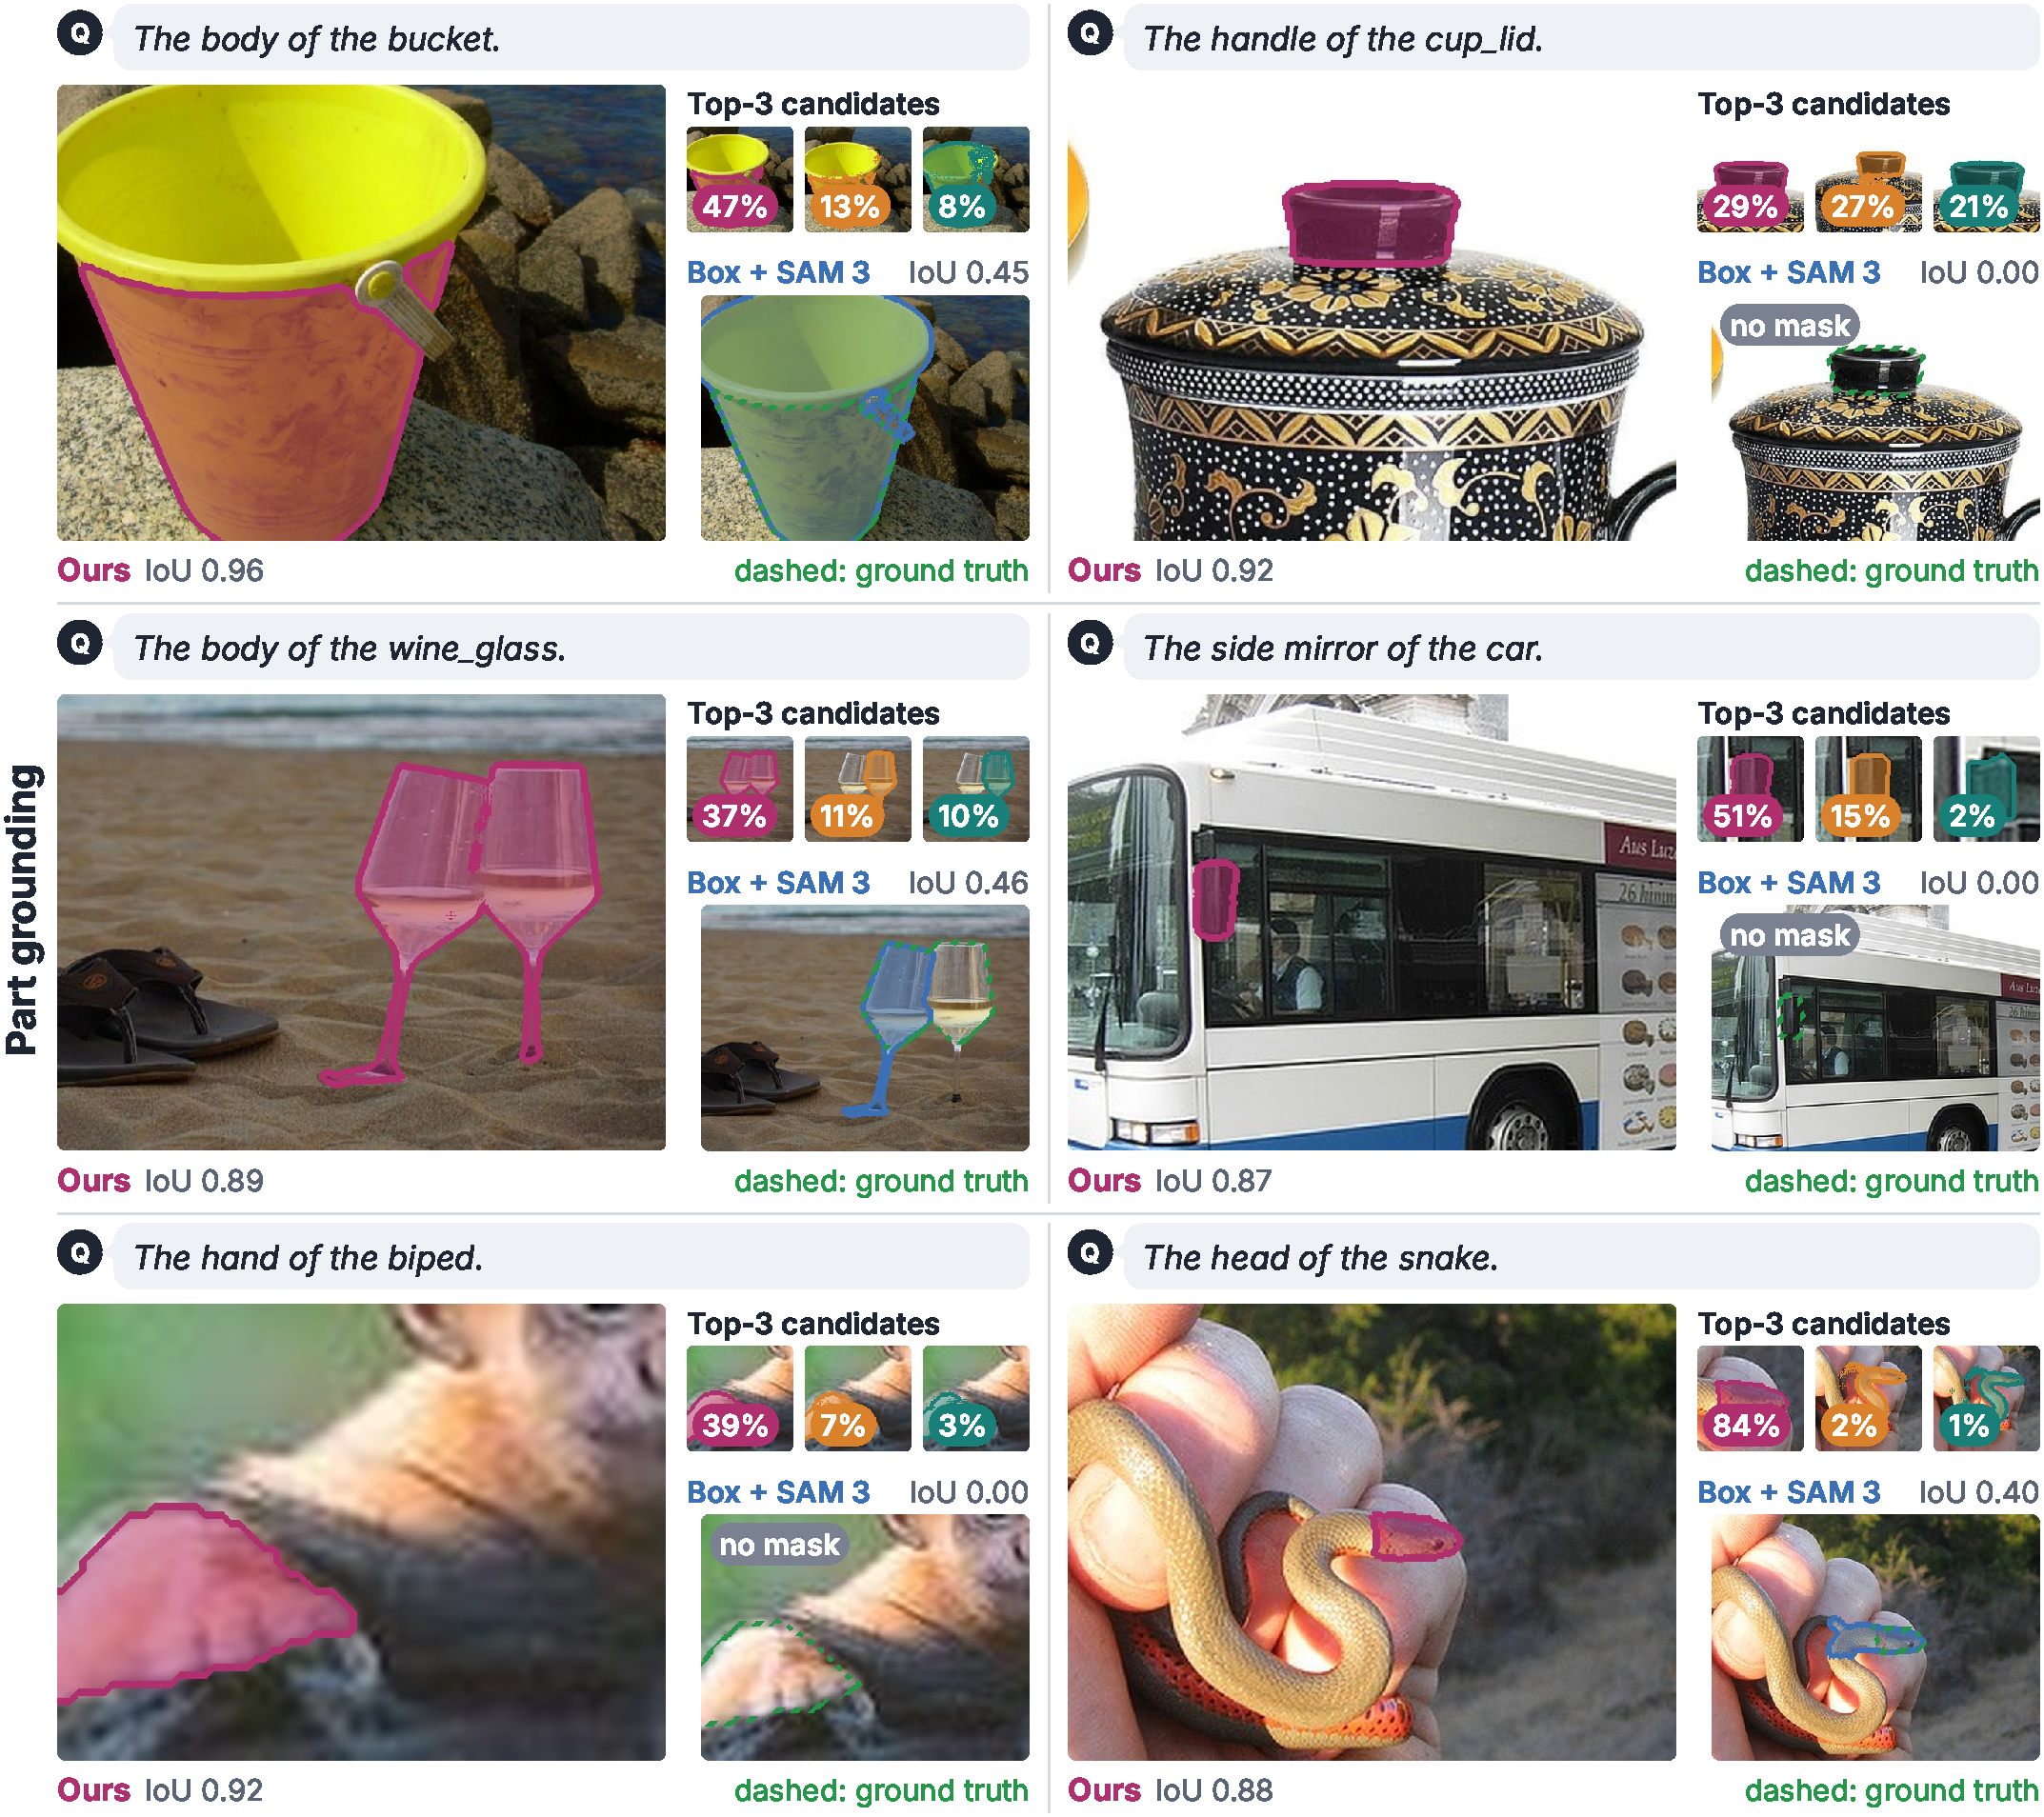
\includegraphics[width=\textwidth,height=0.9\textheight,keepaspectratio]{figures/qualitative/supp/part_selected_1.pdf}
\caption{\textbf{Part grounding: selected examples (1/3).} Test examples where \ours{} clearly beats Box + SAM\,3, in the format of Fig.~\ref{fig:showcase}; none of them appears in the main paper. Filled magenta: the mask \ours{} selects; blue: baselines; dashed green: ground truth.}
\label{fig:supp_part_selected_1}
\end{figure*}

\begin{figure*}[p]
\centering
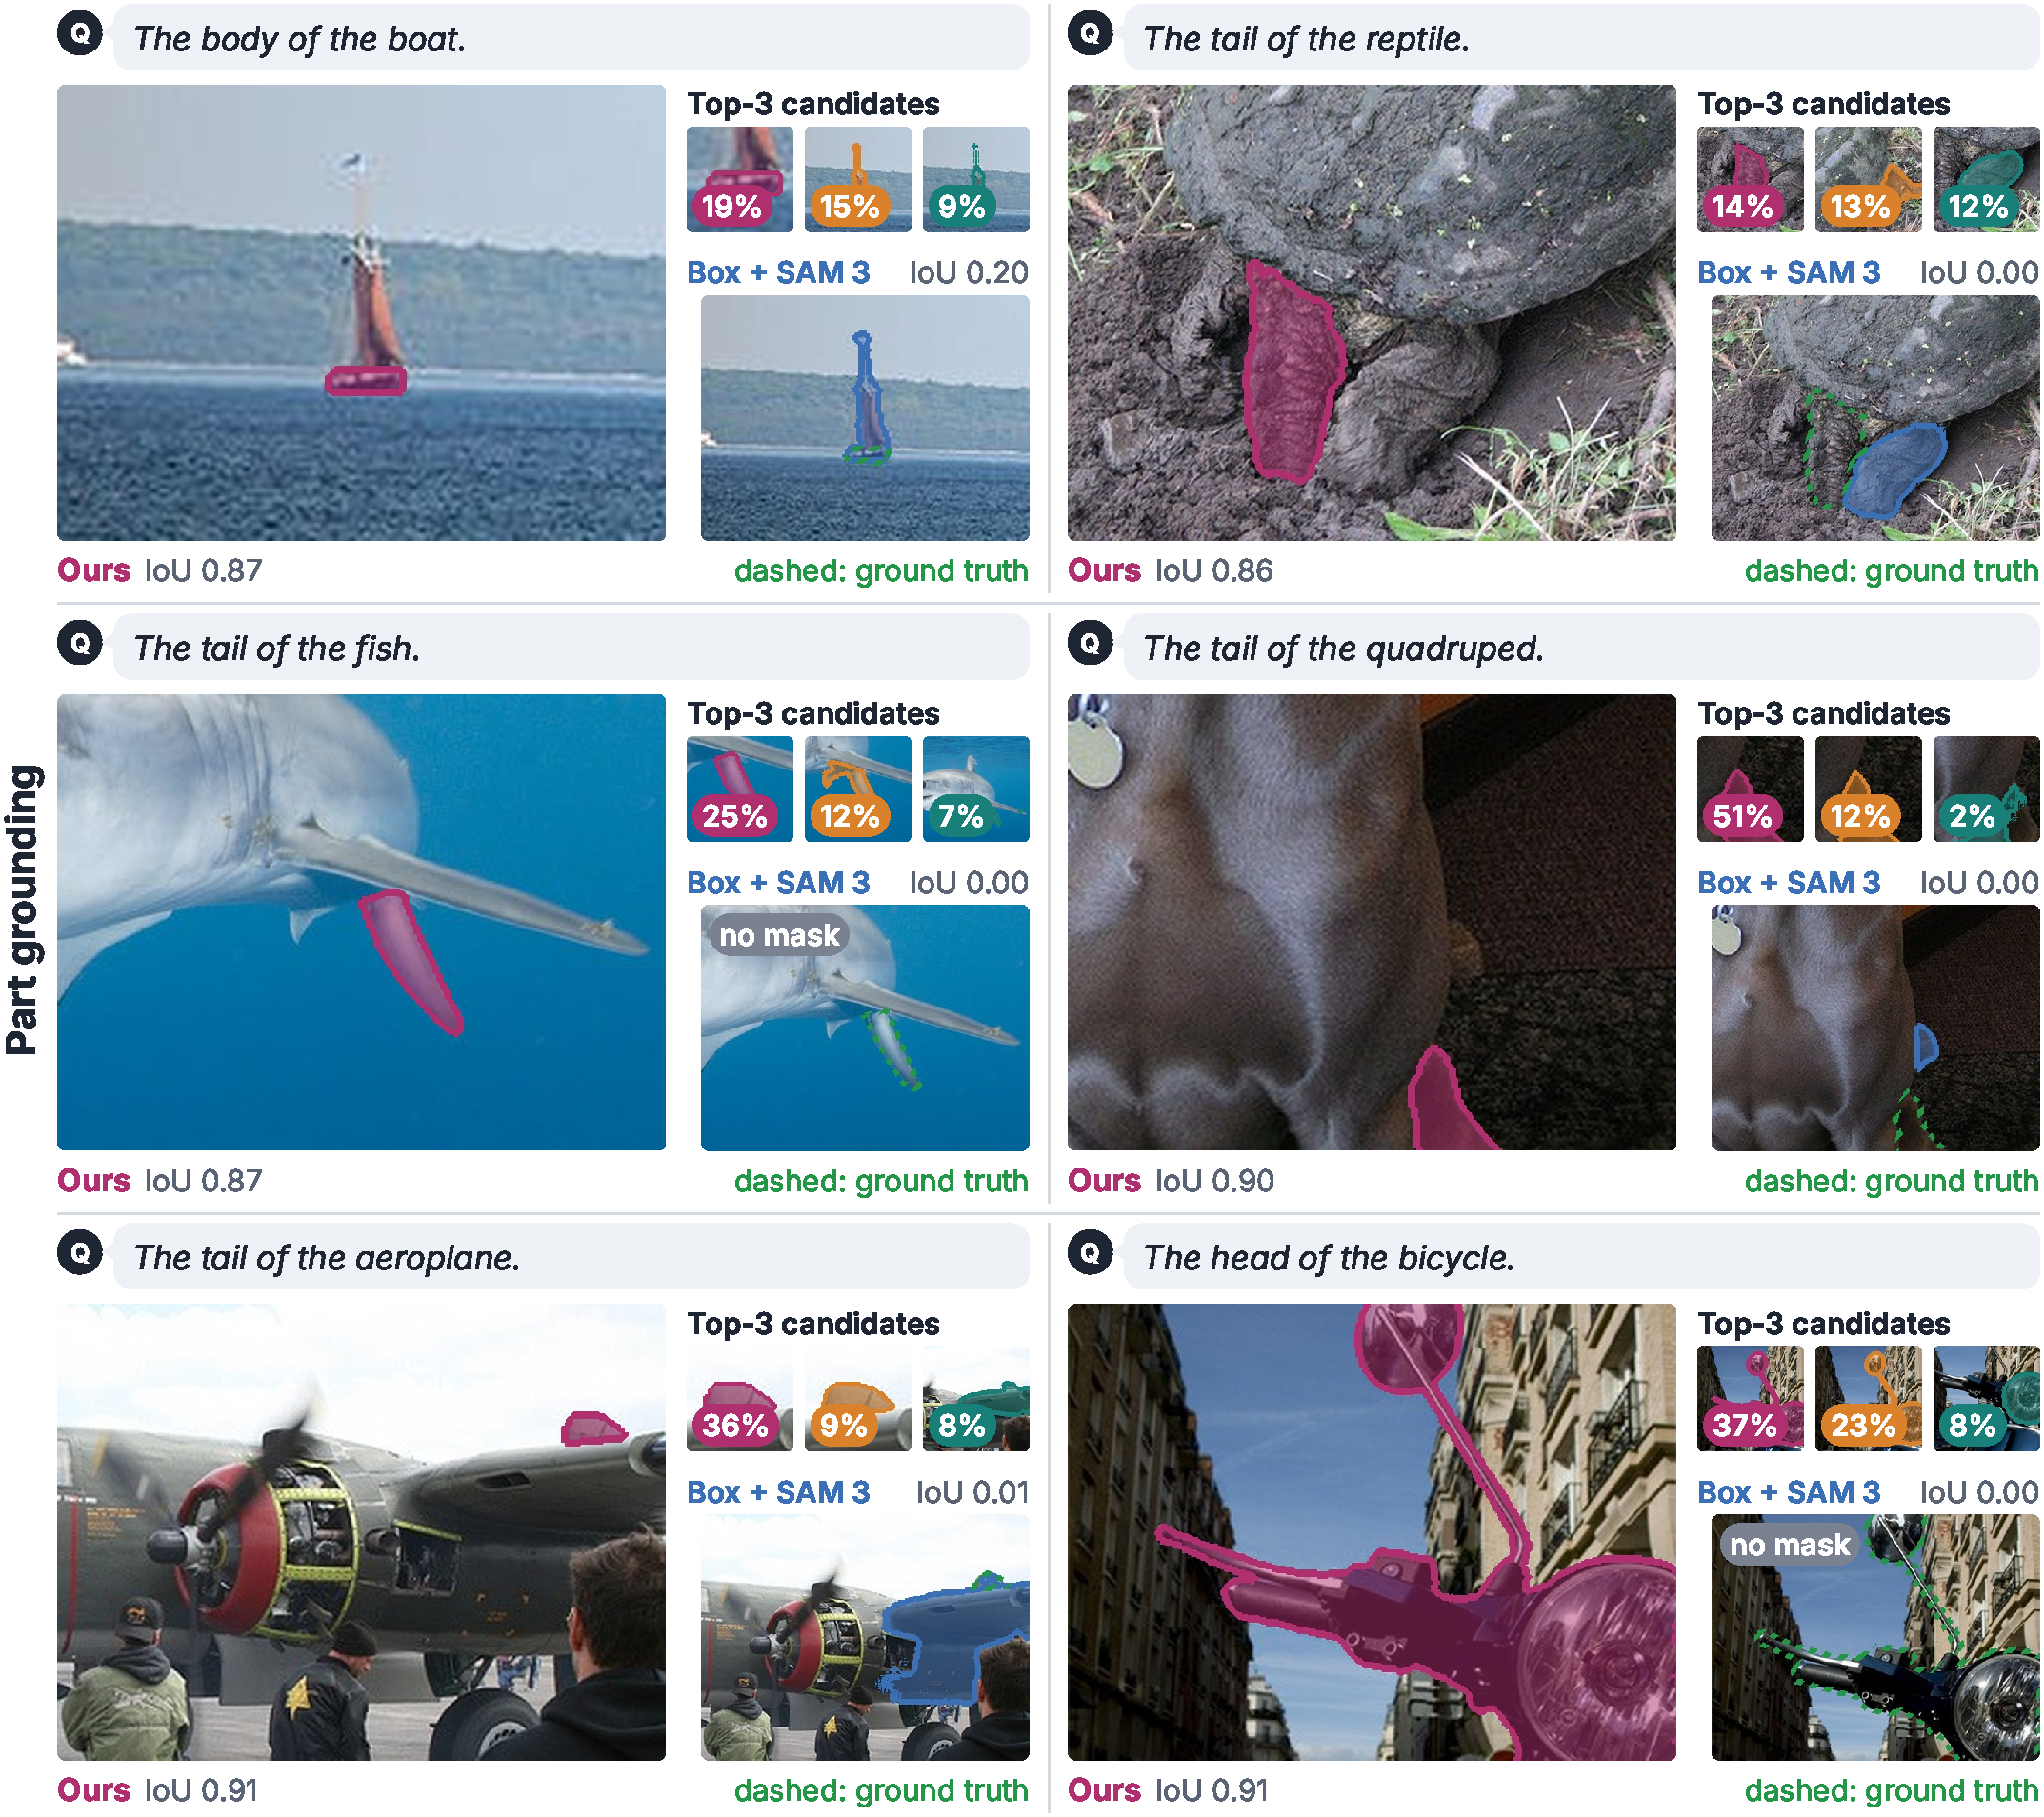
\includegraphics[width=\textwidth,height=0.9\textheight,keepaspectratio]{figures/qualitative/supp/part_selected_2.pdf}
\caption{\textbf{Part grounding: selected examples (2/3).} Test examples where \ours{} clearly beats Box + SAM\,3, in the format of Fig.~\ref{fig:showcase}; none of them appears in the main paper. Filled magenta: the mask \ours{} selects; blue: baselines; dashed green: ground truth.}
\label{fig:supp_part_selected_2}
\end{figure*}

\begin{figure*}[p]
\centering
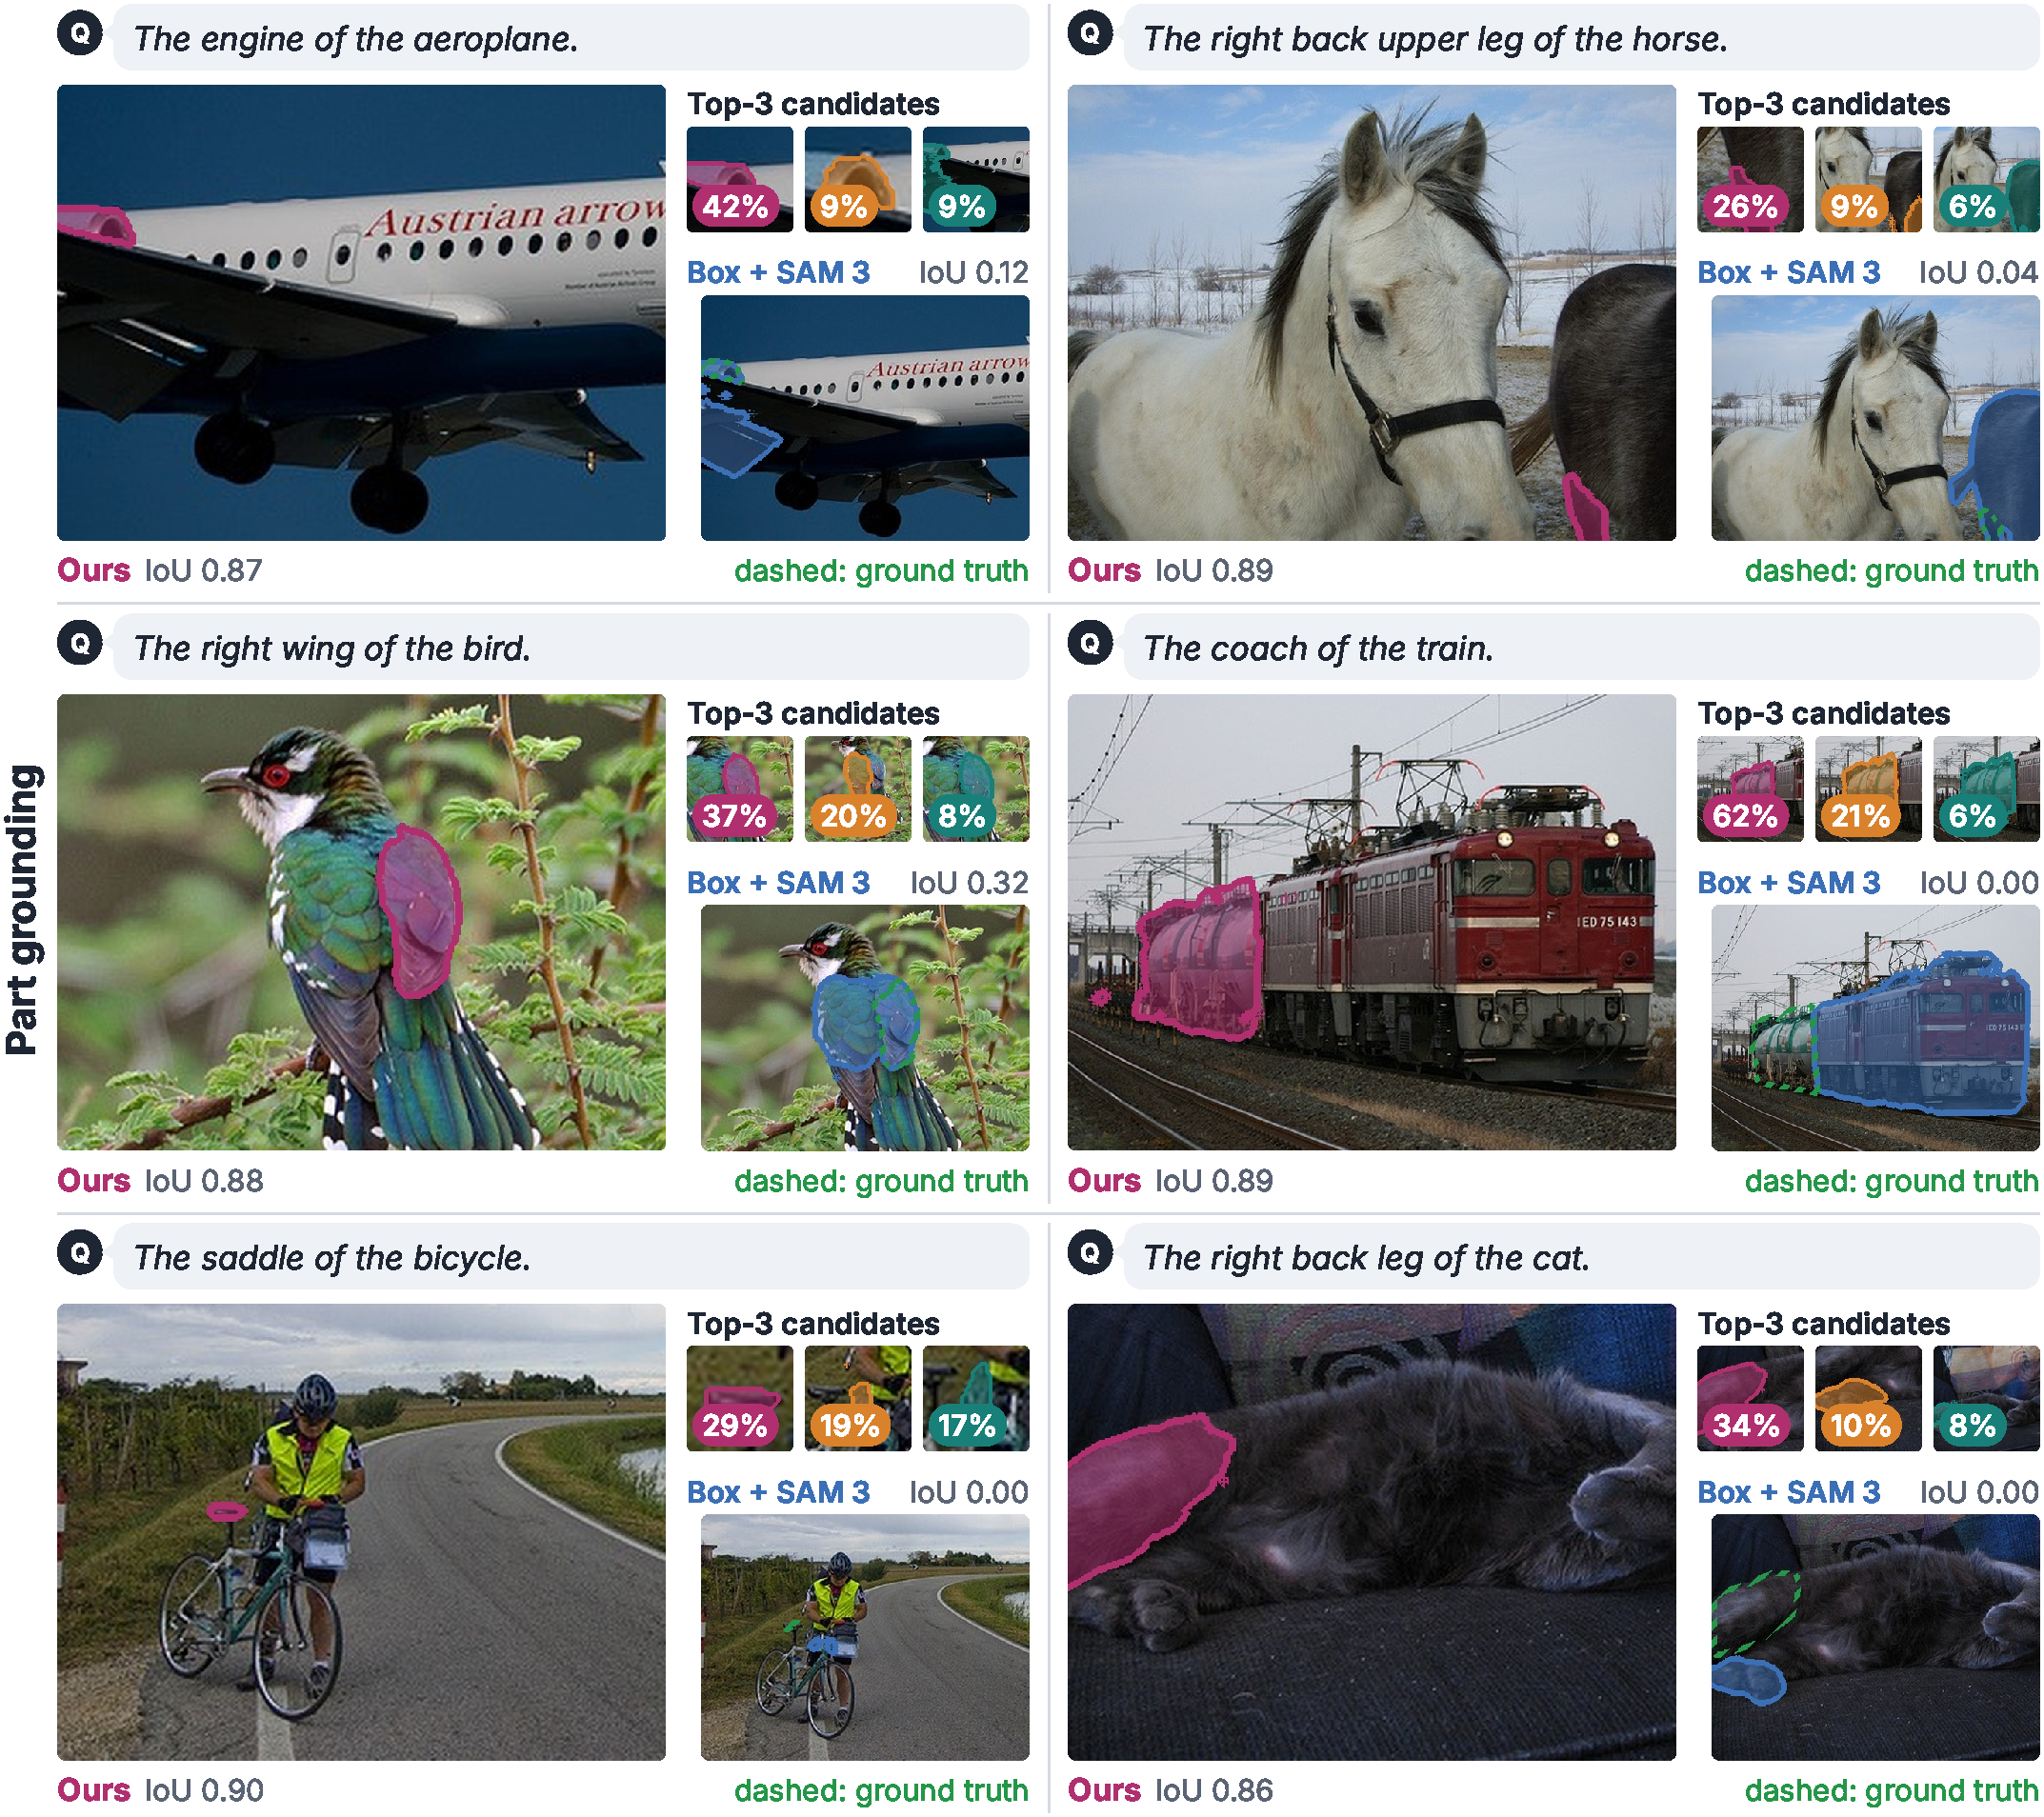
\includegraphics[width=\textwidth,height=0.9\textheight,keepaspectratio]{figures/qualitative/supp/part_selected_3.pdf}
\caption{\textbf{Part grounding: selected examples (3/3).} Test examples where \ours{} clearly beats Box + SAM\,3, in the format of Fig.~\ref{fig:showcase}; none of them appears in the main paper. Filled magenta: the mask \ours{} selects; blue: baselines; dashed green: ground truth.}
\label{fig:supp_part_selected_3}
\end{figure*}

\begin{figure*}[p]
\centering
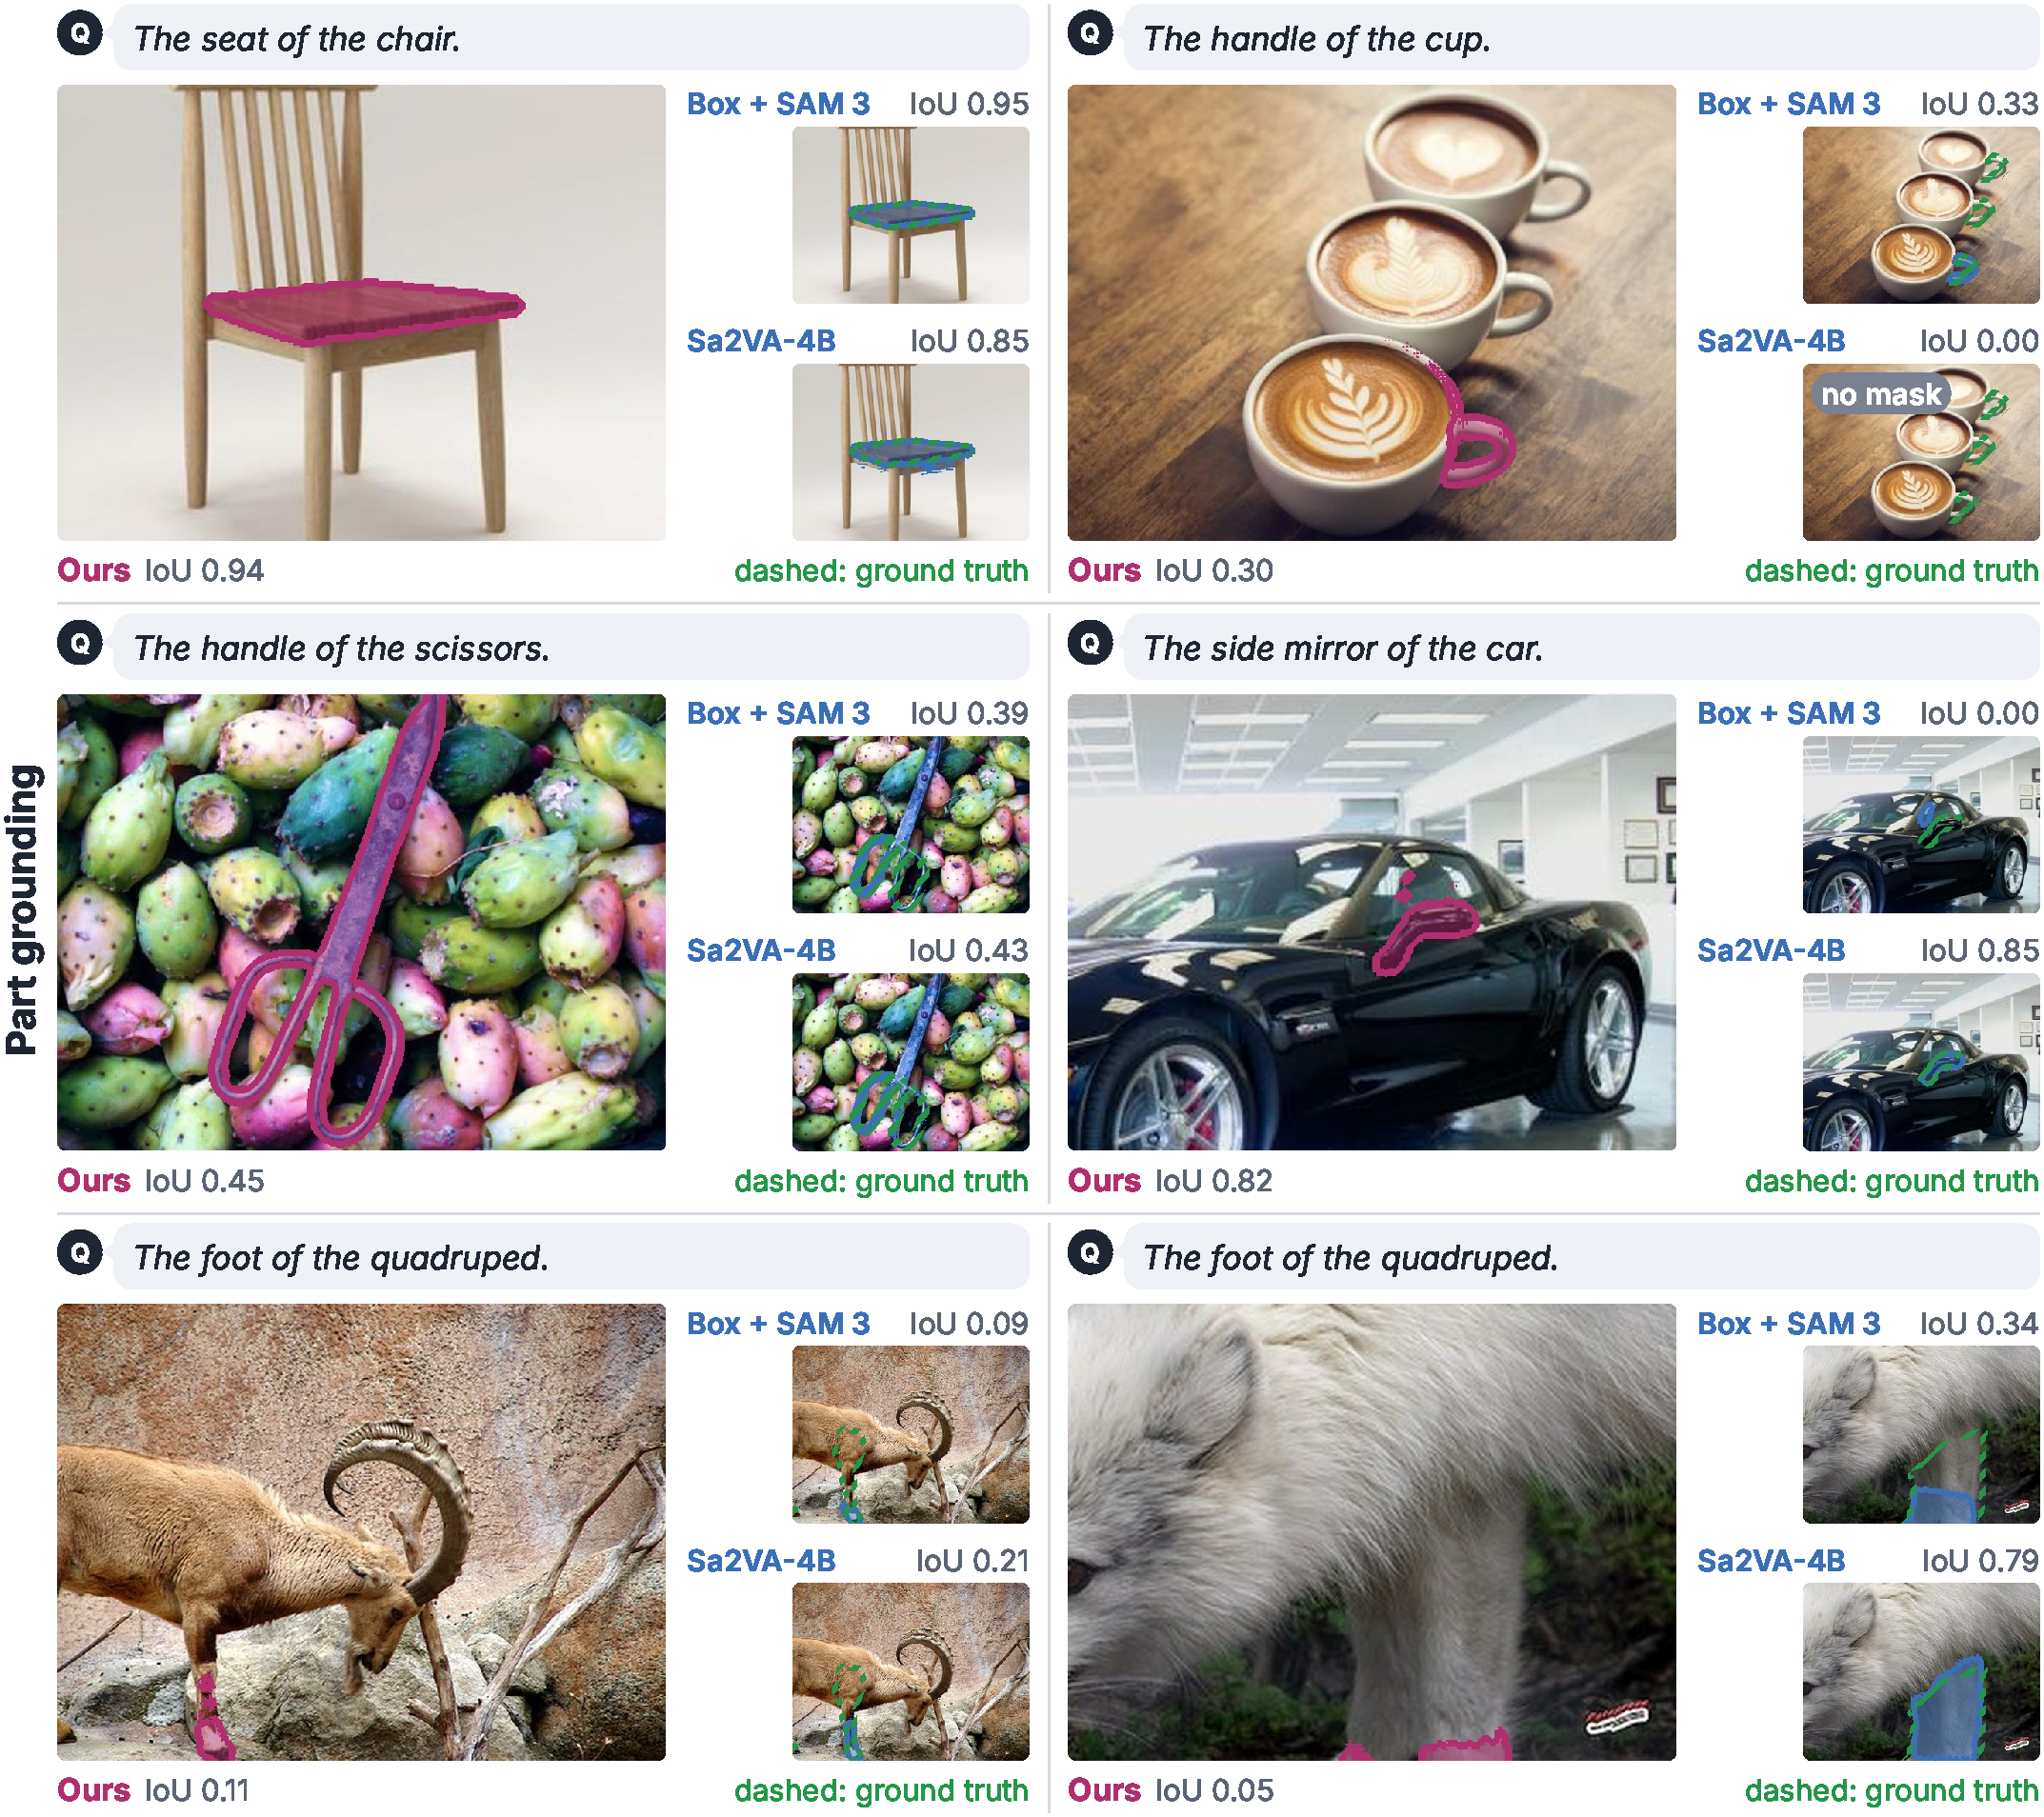
\includegraphics[width=\textwidth,height=0.9\textheight,keepaspectratio]{figures/qualitative/supp/part_random.pdf}
\caption{\textbf{Part grounding: random examples.} A fixed-seed random sample of test queries, not selected for outcome. Filled magenta: the mask \ours{} selects; blue: baselines; dashed green: ground truth.}
\label{fig:supp_part_random}
\end{figure*}

\begin{figure*}[p]
\centering
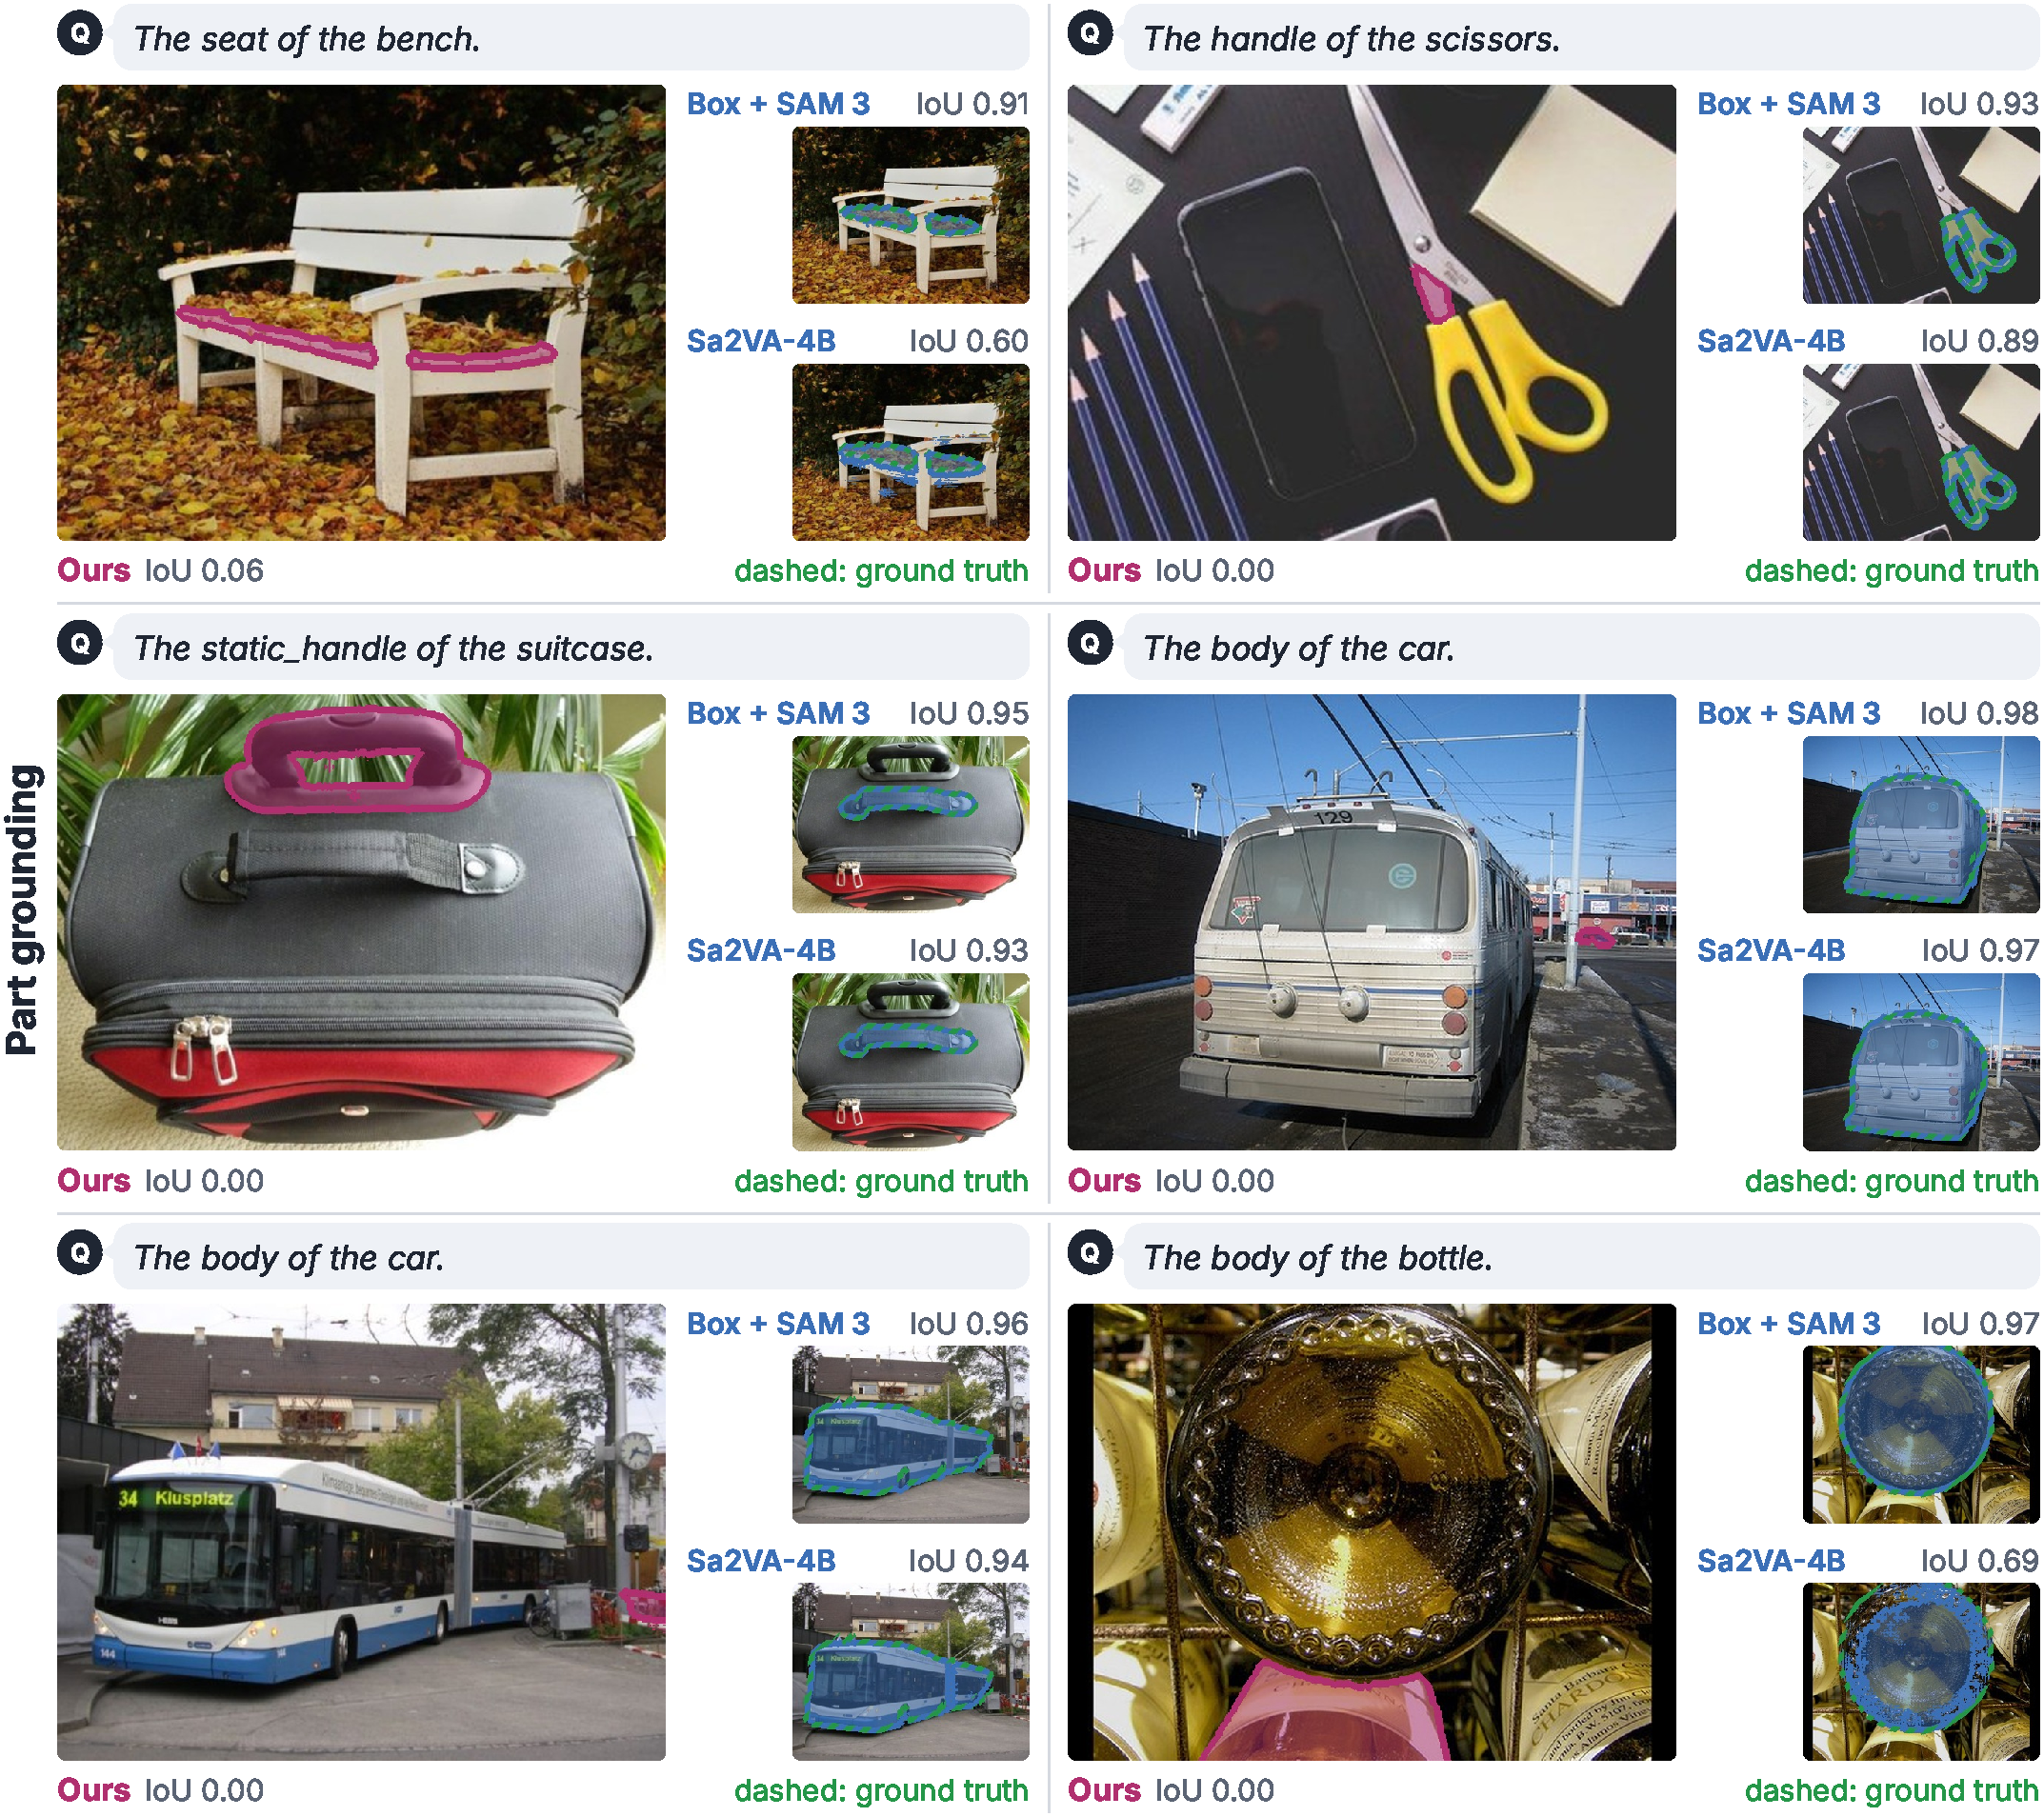
\includegraphics[width=\textwidth,height=0.9\textheight,keepaspectratio]{figures/qualitative/supp/part_failures.pdf}
\caption{\textbf{Part grounding: failure cases.} The test queries where \ours{} falls furthest behind Box + SAM\,3. Filled magenta: the mask \ours{} selects; blue: baselines; dashed green: ground truth.}
\label{fig:supp_part_failures}
\end{figure*}

\begin{figure*}[p]
\centering
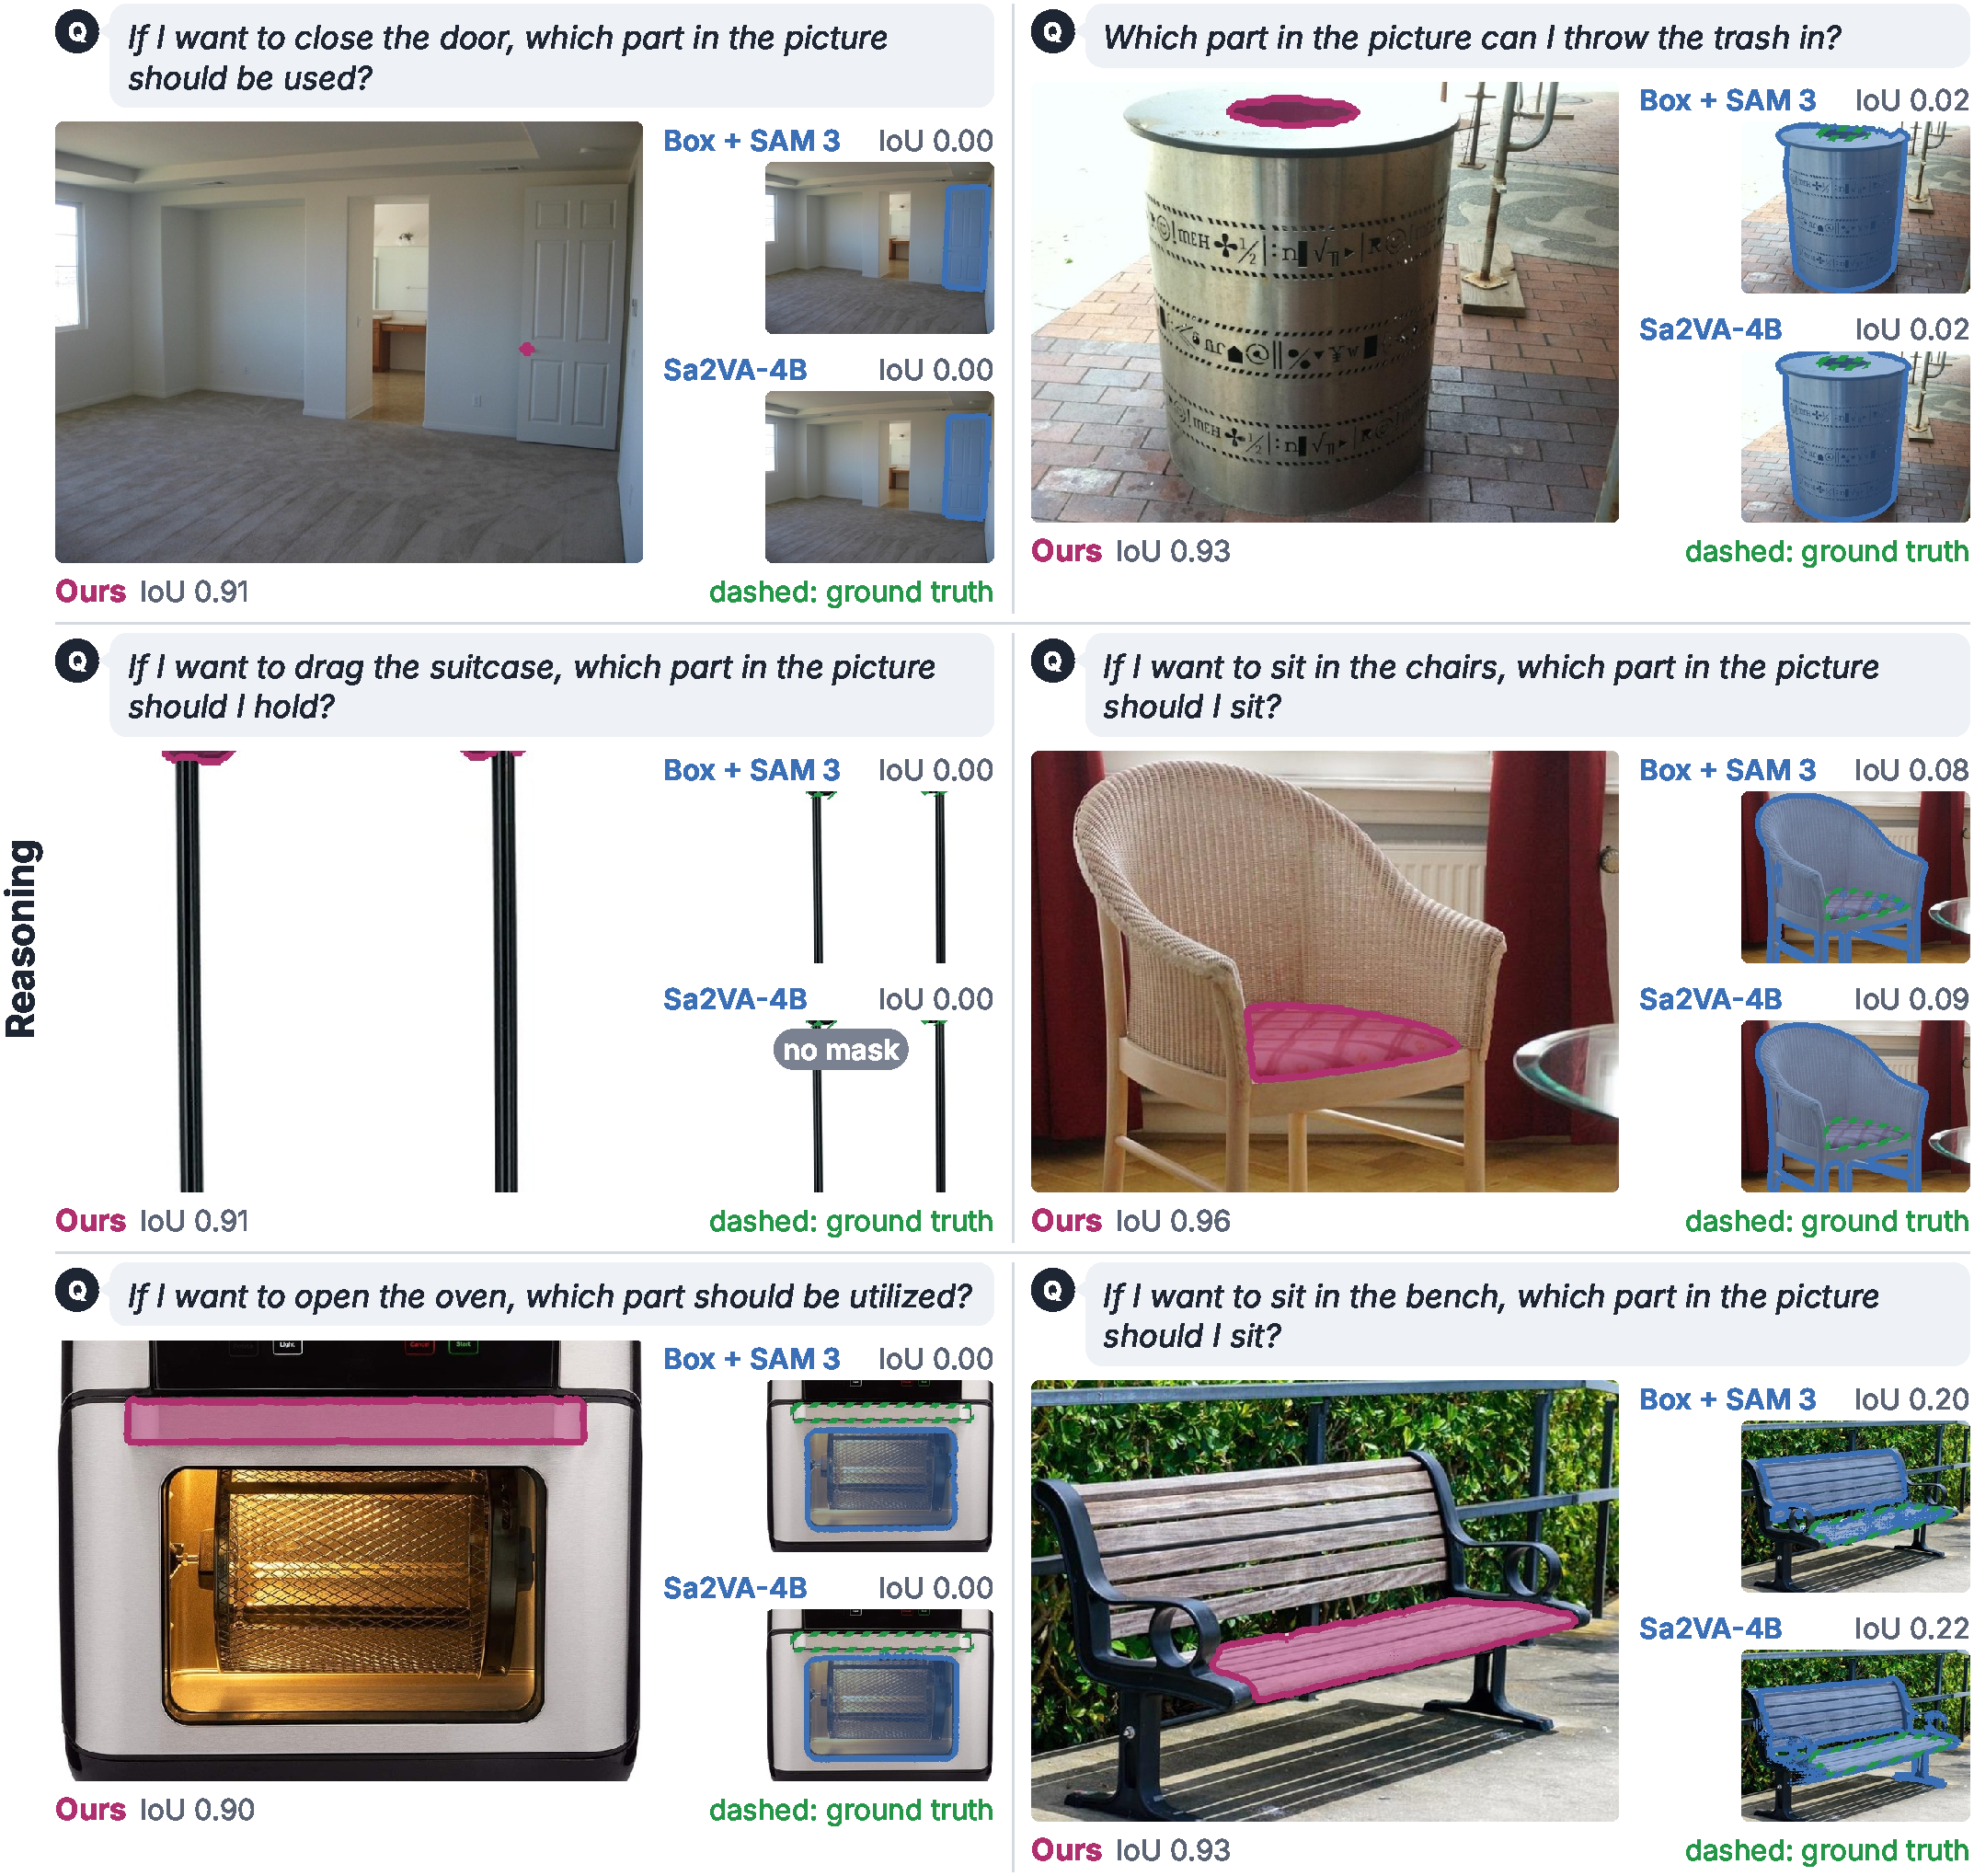
\includegraphics[width=\textwidth,height=0.9\textheight,keepaspectratio]{figures/qualitative/supp/reason_selected_1.pdf}
\caption{\textbf{Reasoning: selected examples (1/3).} Test examples where \ours{} clearly beats Box + SAM\,3, in the format of Fig.~\ref{fig:showcase}; none of them appears in the main paper. Selected examples use query rewriting; random examples and failure cases show \ours{} without it.}
\label{fig:supp_reason_selected_1}
\end{figure*}

\begin{figure*}[p]
\centering
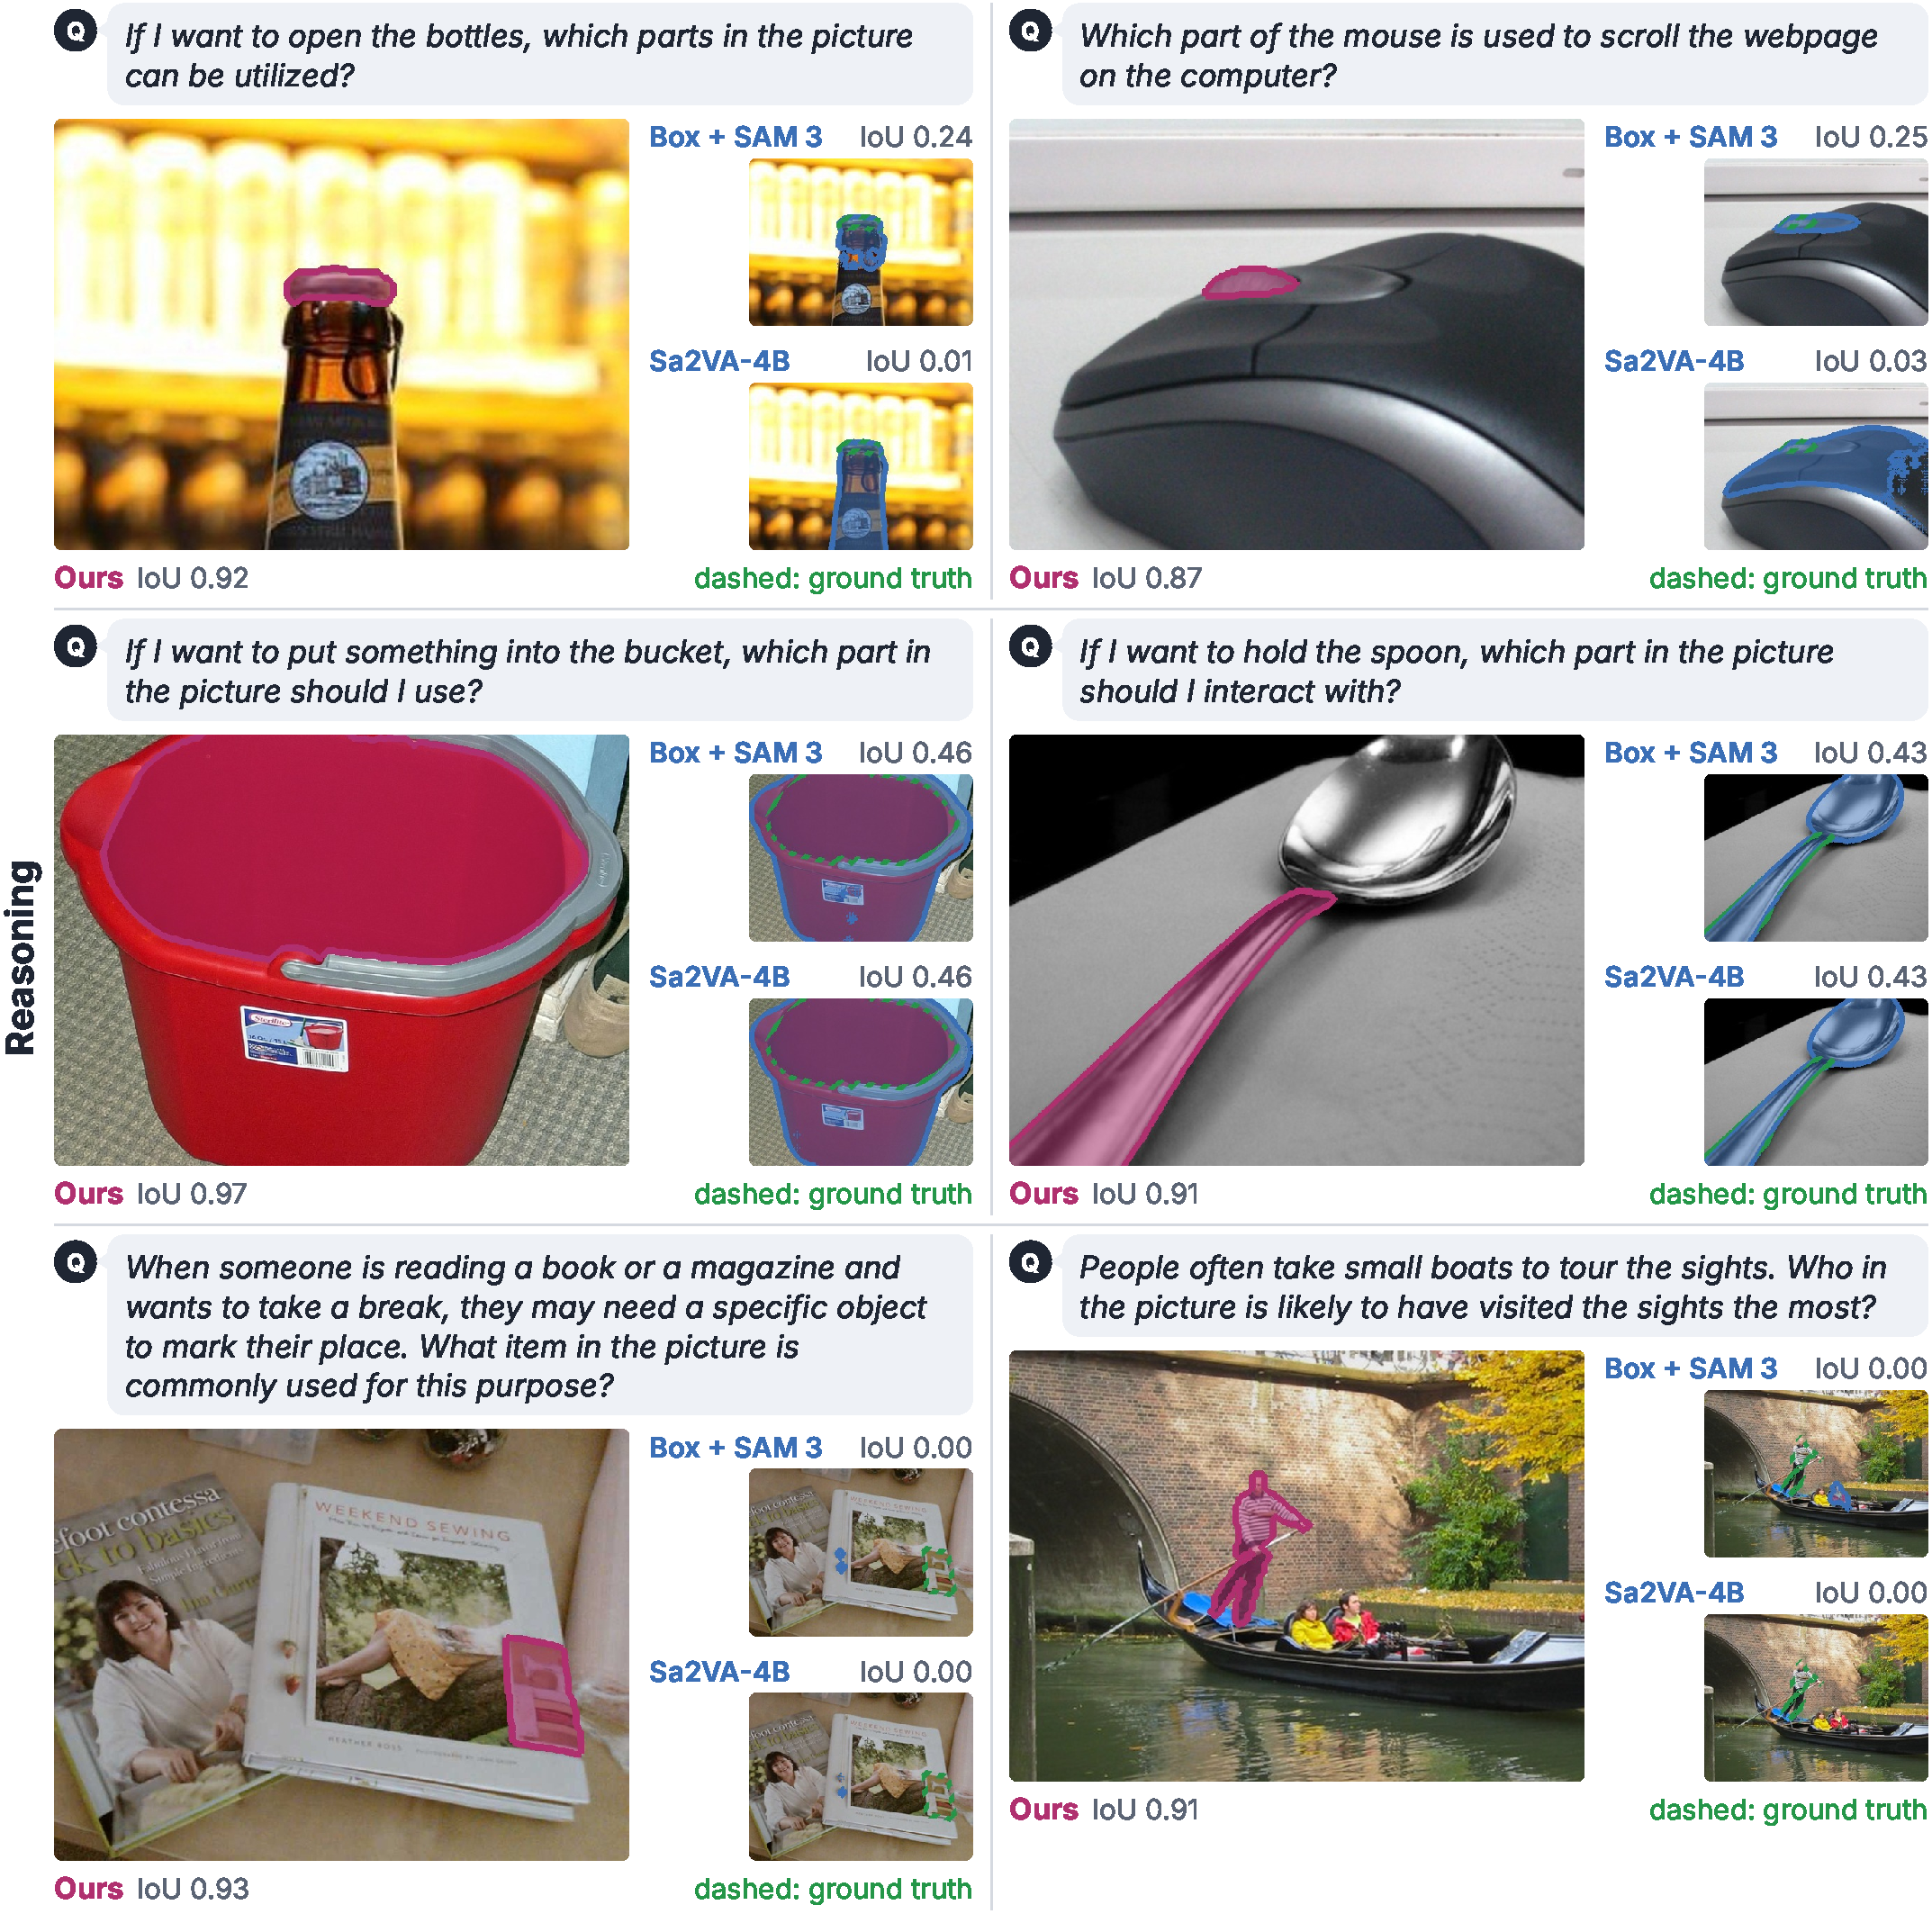
\includegraphics[width=\textwidth,height=0.9\textheight,keepaspectratio]{figures/qualitative/supp/reason_selected_2.pdf}
\caption{\textbf{Reasoning: selected examples (2/3).} Test examples where \ours{} clearly beats Box + SAM\,3, in the format of Fig.~\ref{fig:showcase}; none of them appears in the main paper. Selected examples use query rewriting; random examples and failure cases show \ours{} without it.}
\label{fig:supp_reason_selected_2}
\end{figure*}

\begin{figure*}[p]
\centering
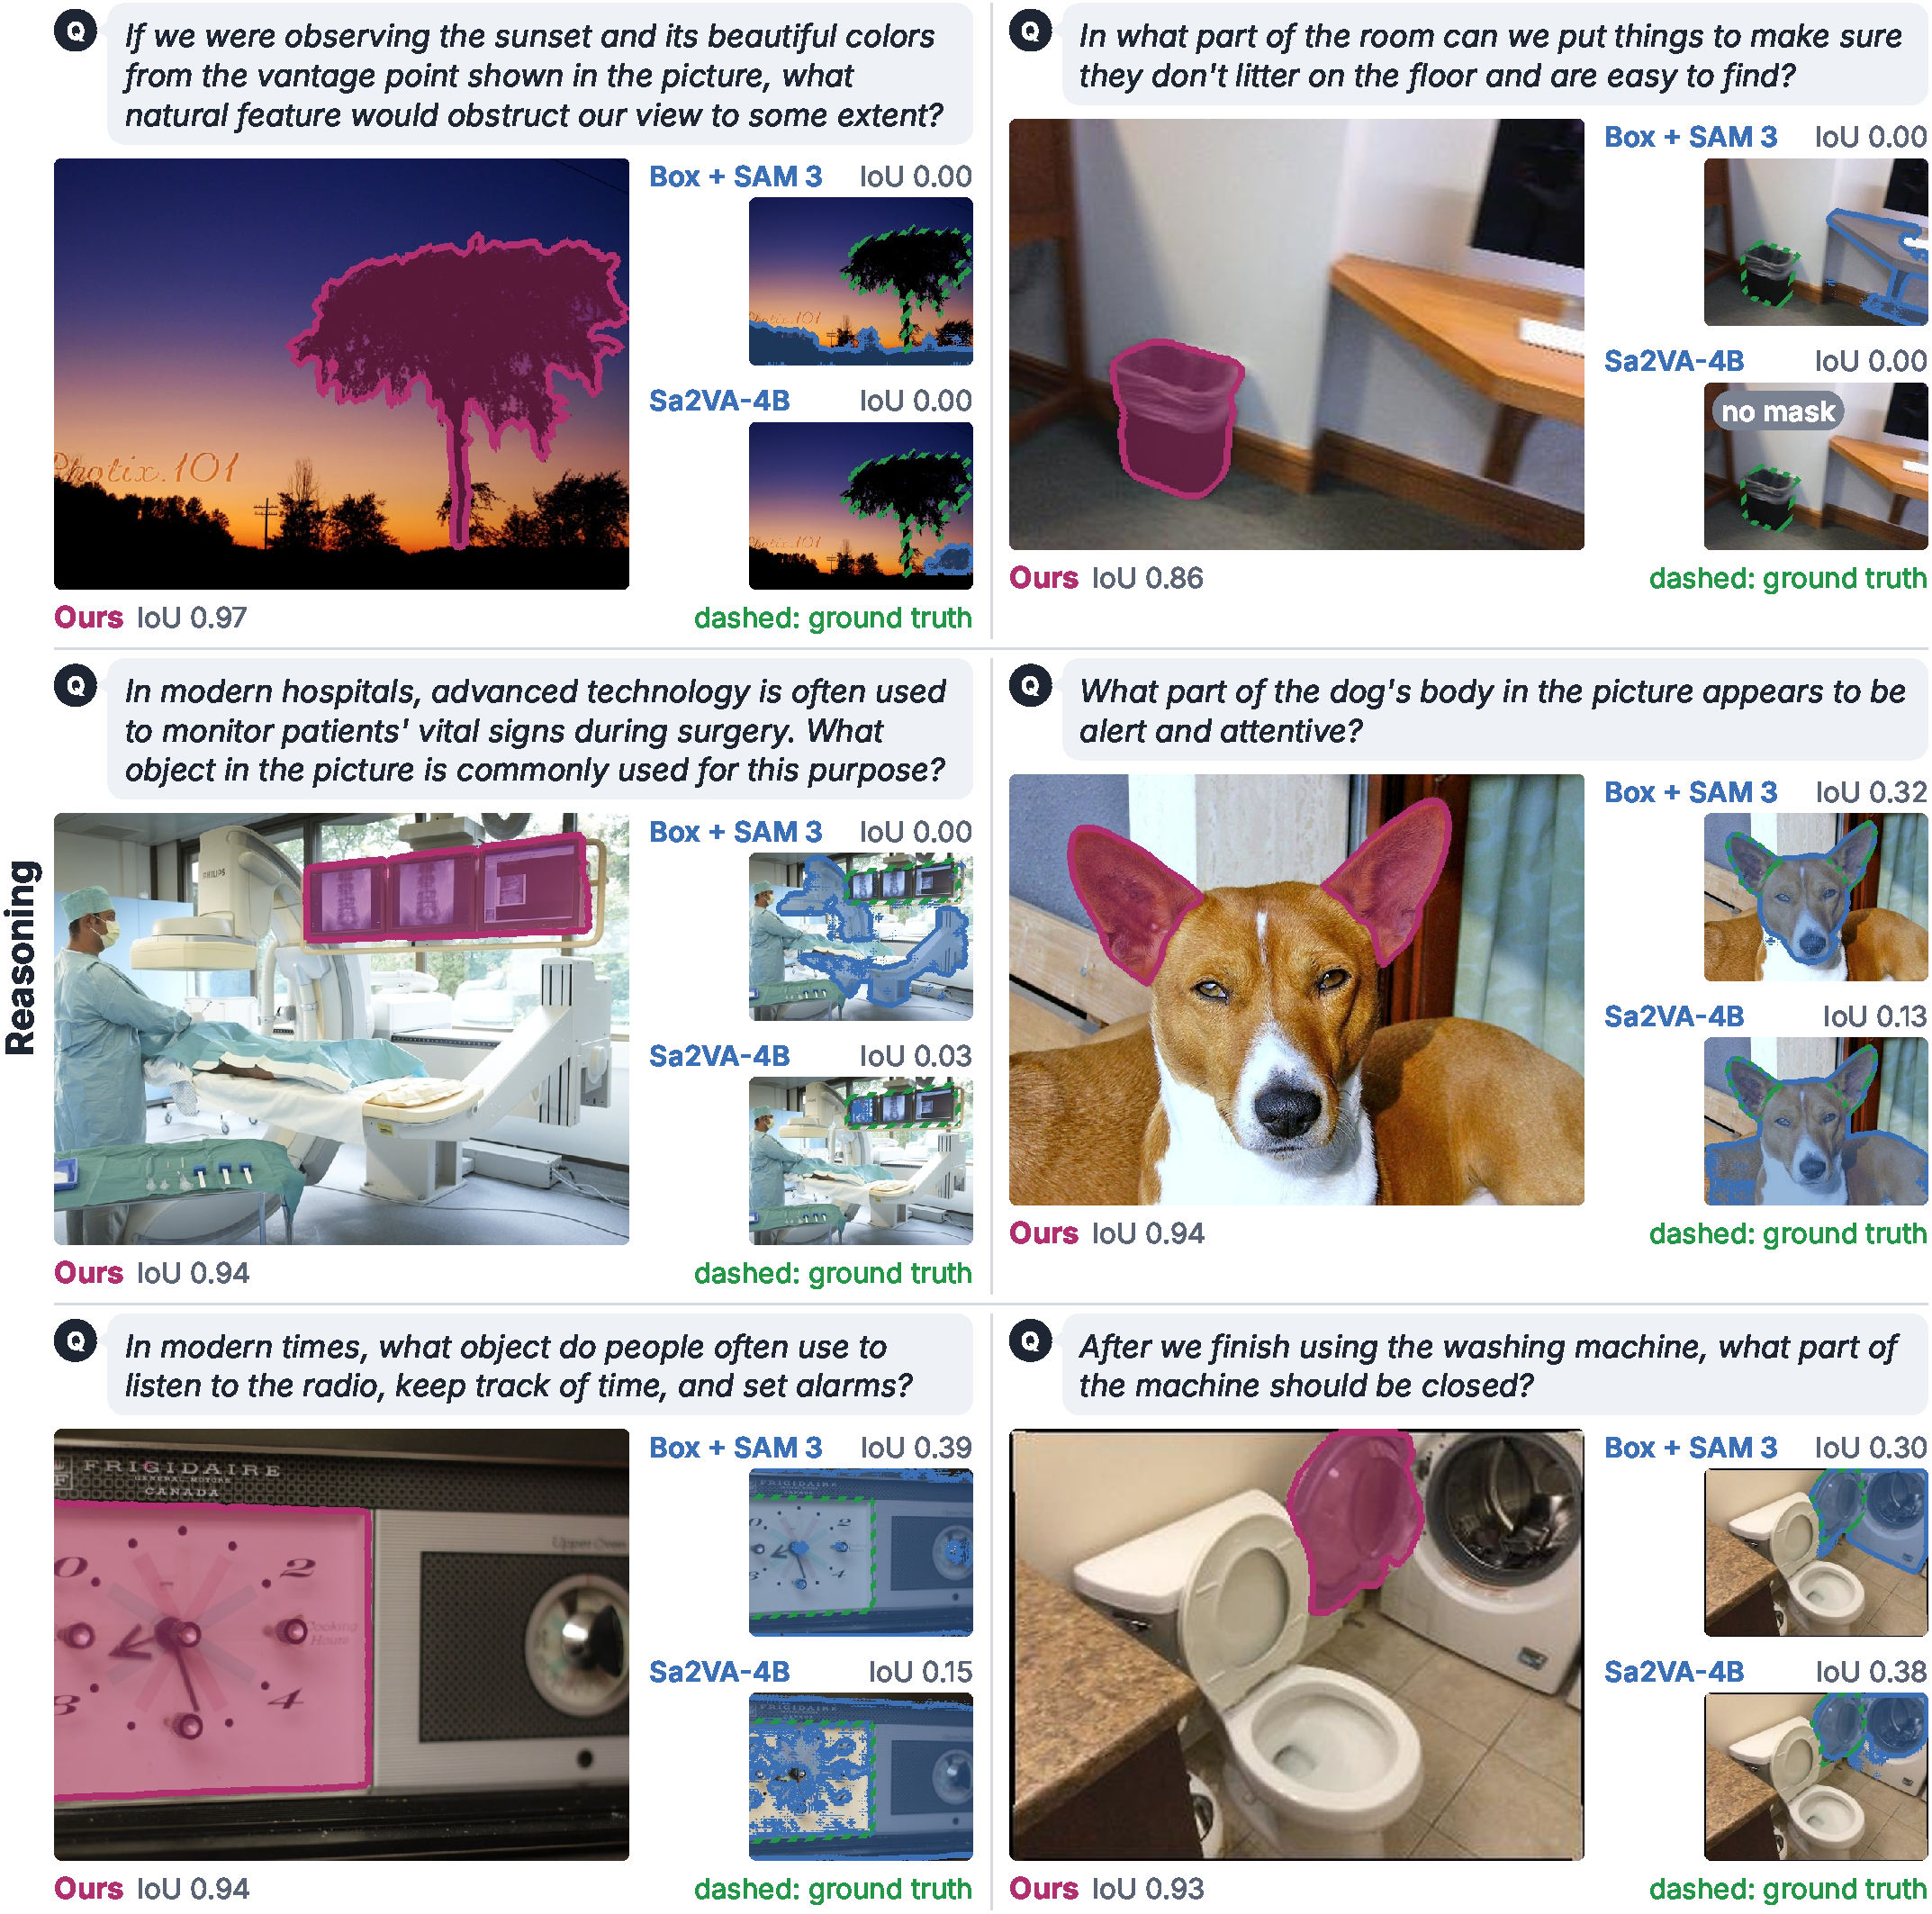
\includegraphics[width=\textwidth,height=0.9\textheight,keepaspectratio]{figures/qualitative/supp/reason_selected_3.pdf}
\caption{\textbf{Reasoning: selected examples (3/3).} Test examples where \ours{} clearly beats Box + SAM\,3, in the format of Fig.~\ref{fig:showcase}; none of them appears in the main paper. Selected examples use query rewriting; random examples and failure cases show \ours{} without it.}
\label{fig:supp_reason_selected_3}
\end{figure*}

\begin{figure*}[p]
\centering
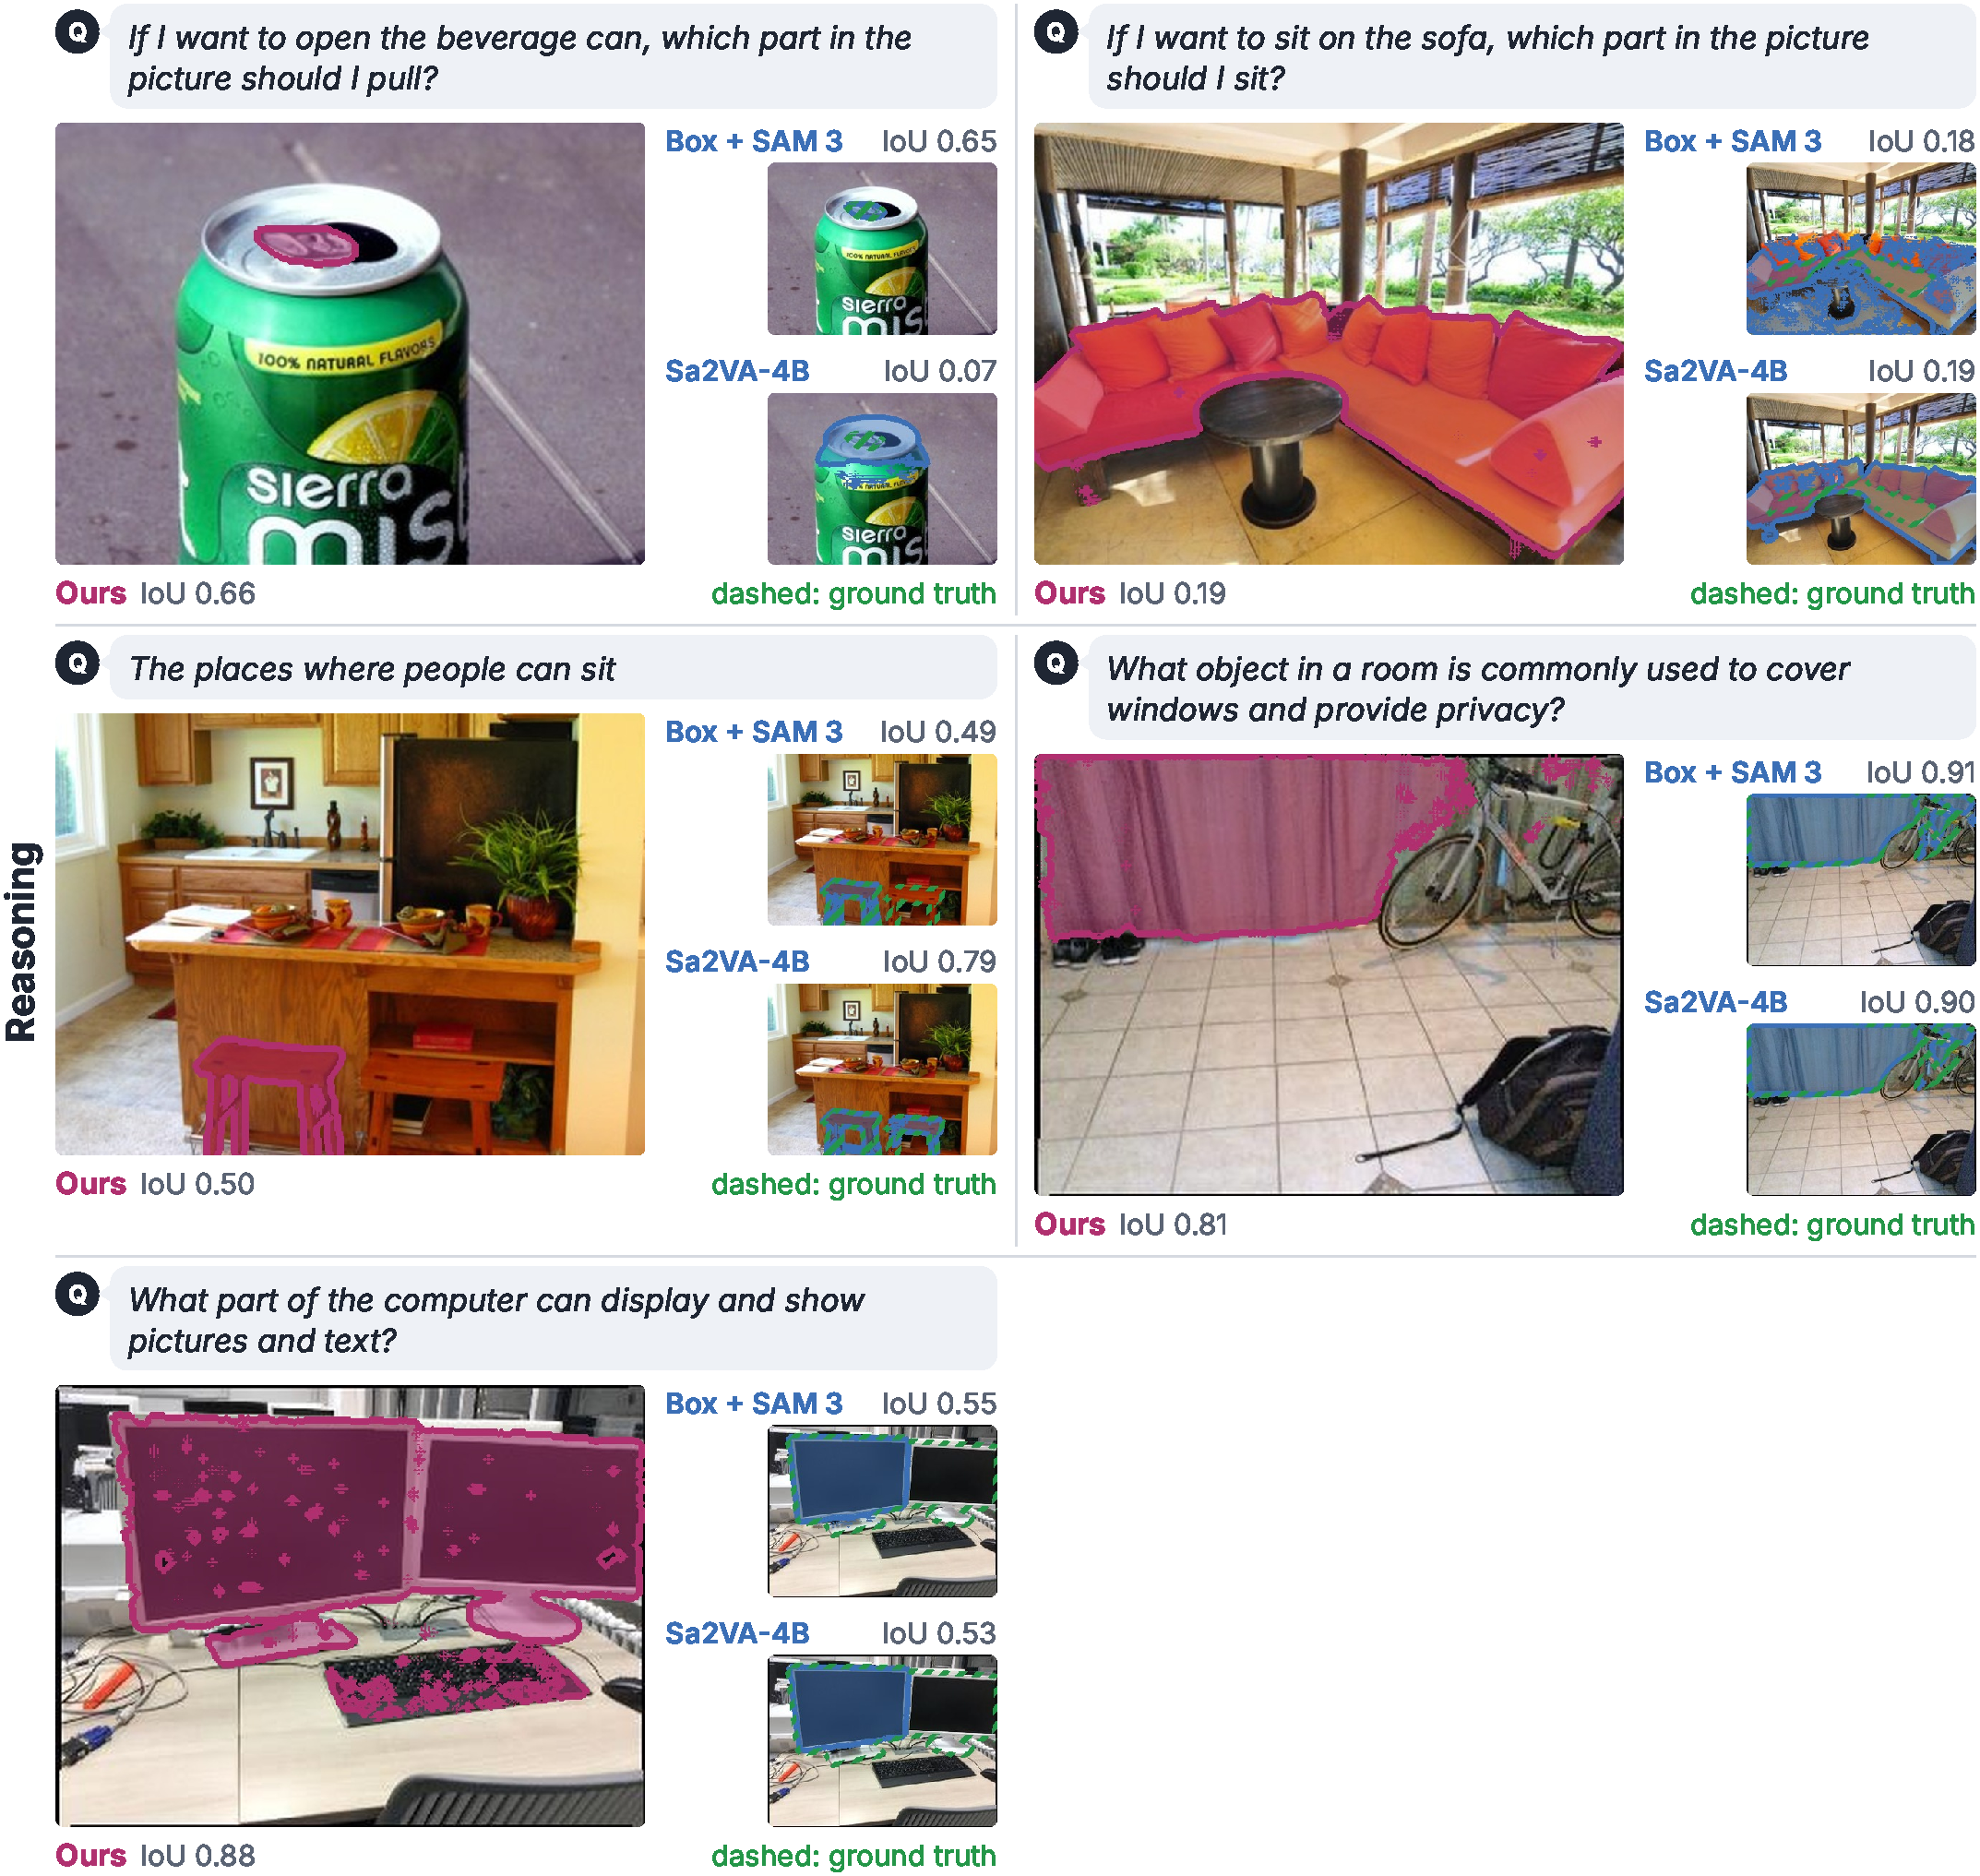
\includegraphics[width=\textwidth,height=0.9\textheight,keepaspectratio]{figures/qualitative/supp/reason_random.pdf}
\caption{\textbf{Reasoning: random examples.} A fixed-seed random sample of test queries, not selected for outcome. Selected examples use query rewriting; random examples and failure cases show \ours{} without it.}
\label{fig:supp_reason_random}
\end{figure*}

\begin{figure*}[p]
\centering
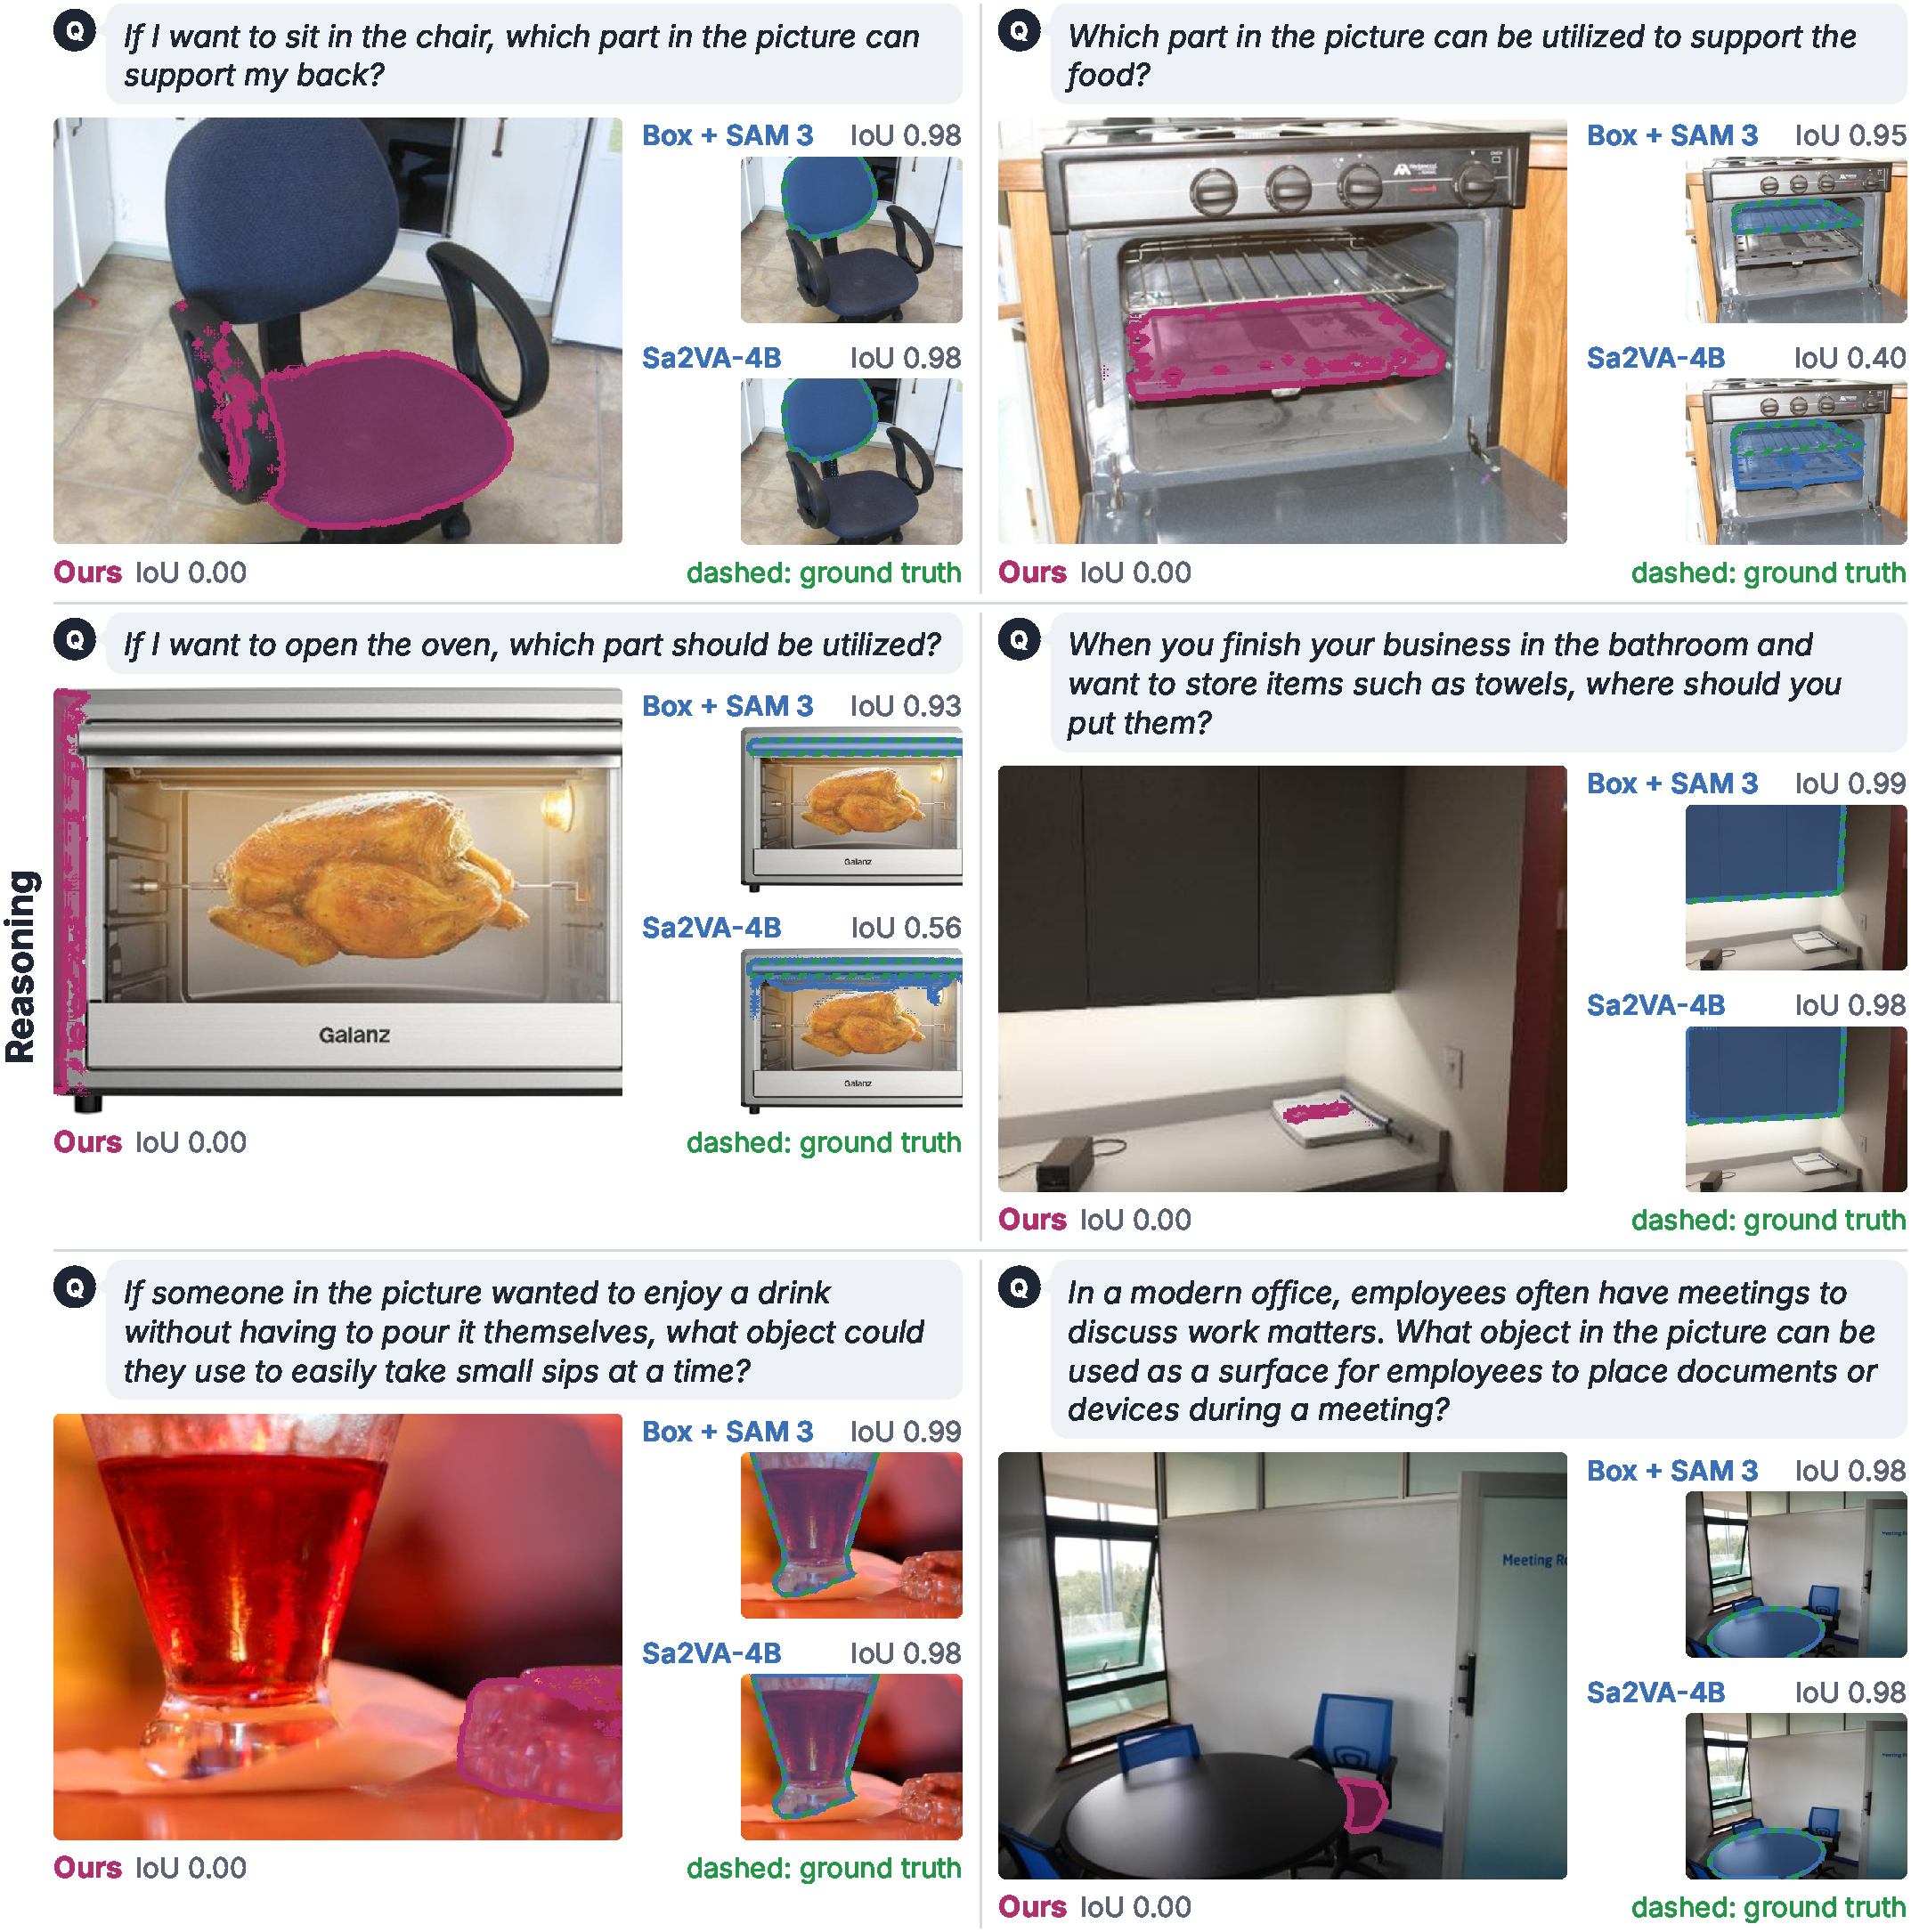
\includegraphics[width=\textwidth,height=0.9\textheight,keepaspectratio]{figures/qualitative/supp/reason_failures.pdf}
\caption{\textbf{Reasoning: failure cases.} The test queries where \ours{} falls furthest behind Box + SAM\,3. Selected examples use query rewriting; random examples and failure cases show \ours{} without it.}
\label{fig:supp_reason_failures}
\end{figure*}

\begin{figure*}[p]
\centering
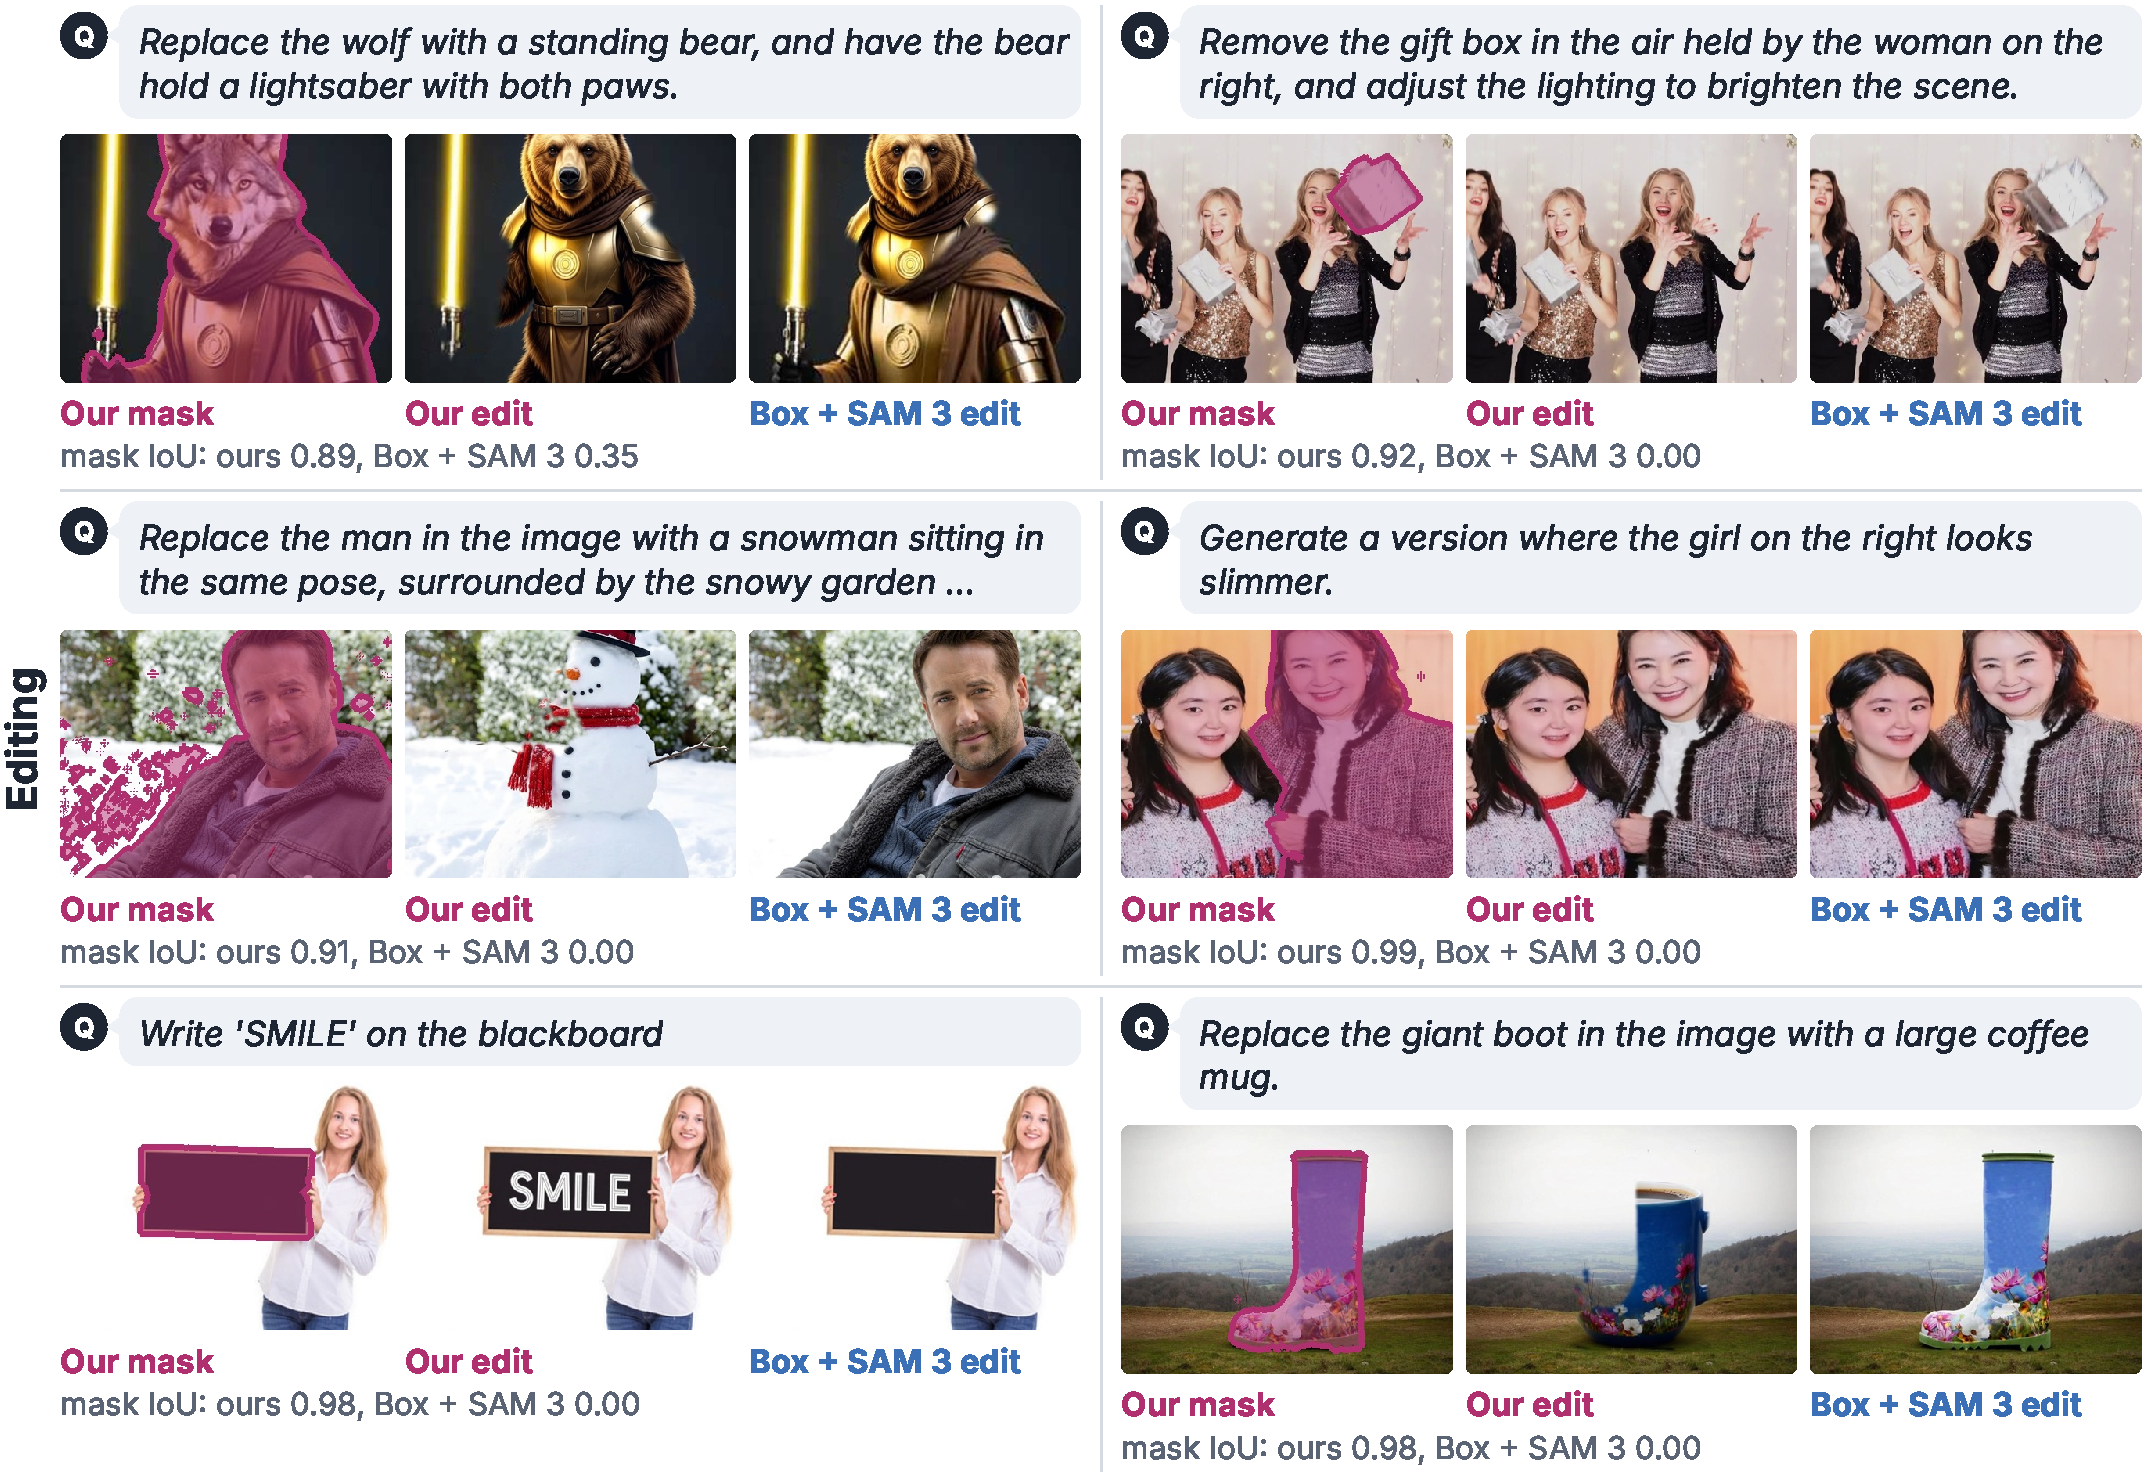
\includegraphics[width=\textwidth,height=0.9\textheight,keepaspectratio]{figures/qualitative/supp/edit_selected_1.pdf}
\caption{\textbf{Editing: selected examples.} Test examples where \ours{} clearly beats Box + SAM\,3, in the format of Fig.~\ref{fig:showcase}; none of them appears in the main paper. Our mask, the edit made with it, and the edit made with the Box + SAM\,3 mask (Qwen-Image-Edit).}
\label{fig:supp_edit_selected_1}
\end{figure*}

\begin{figure*}[p]
\centering
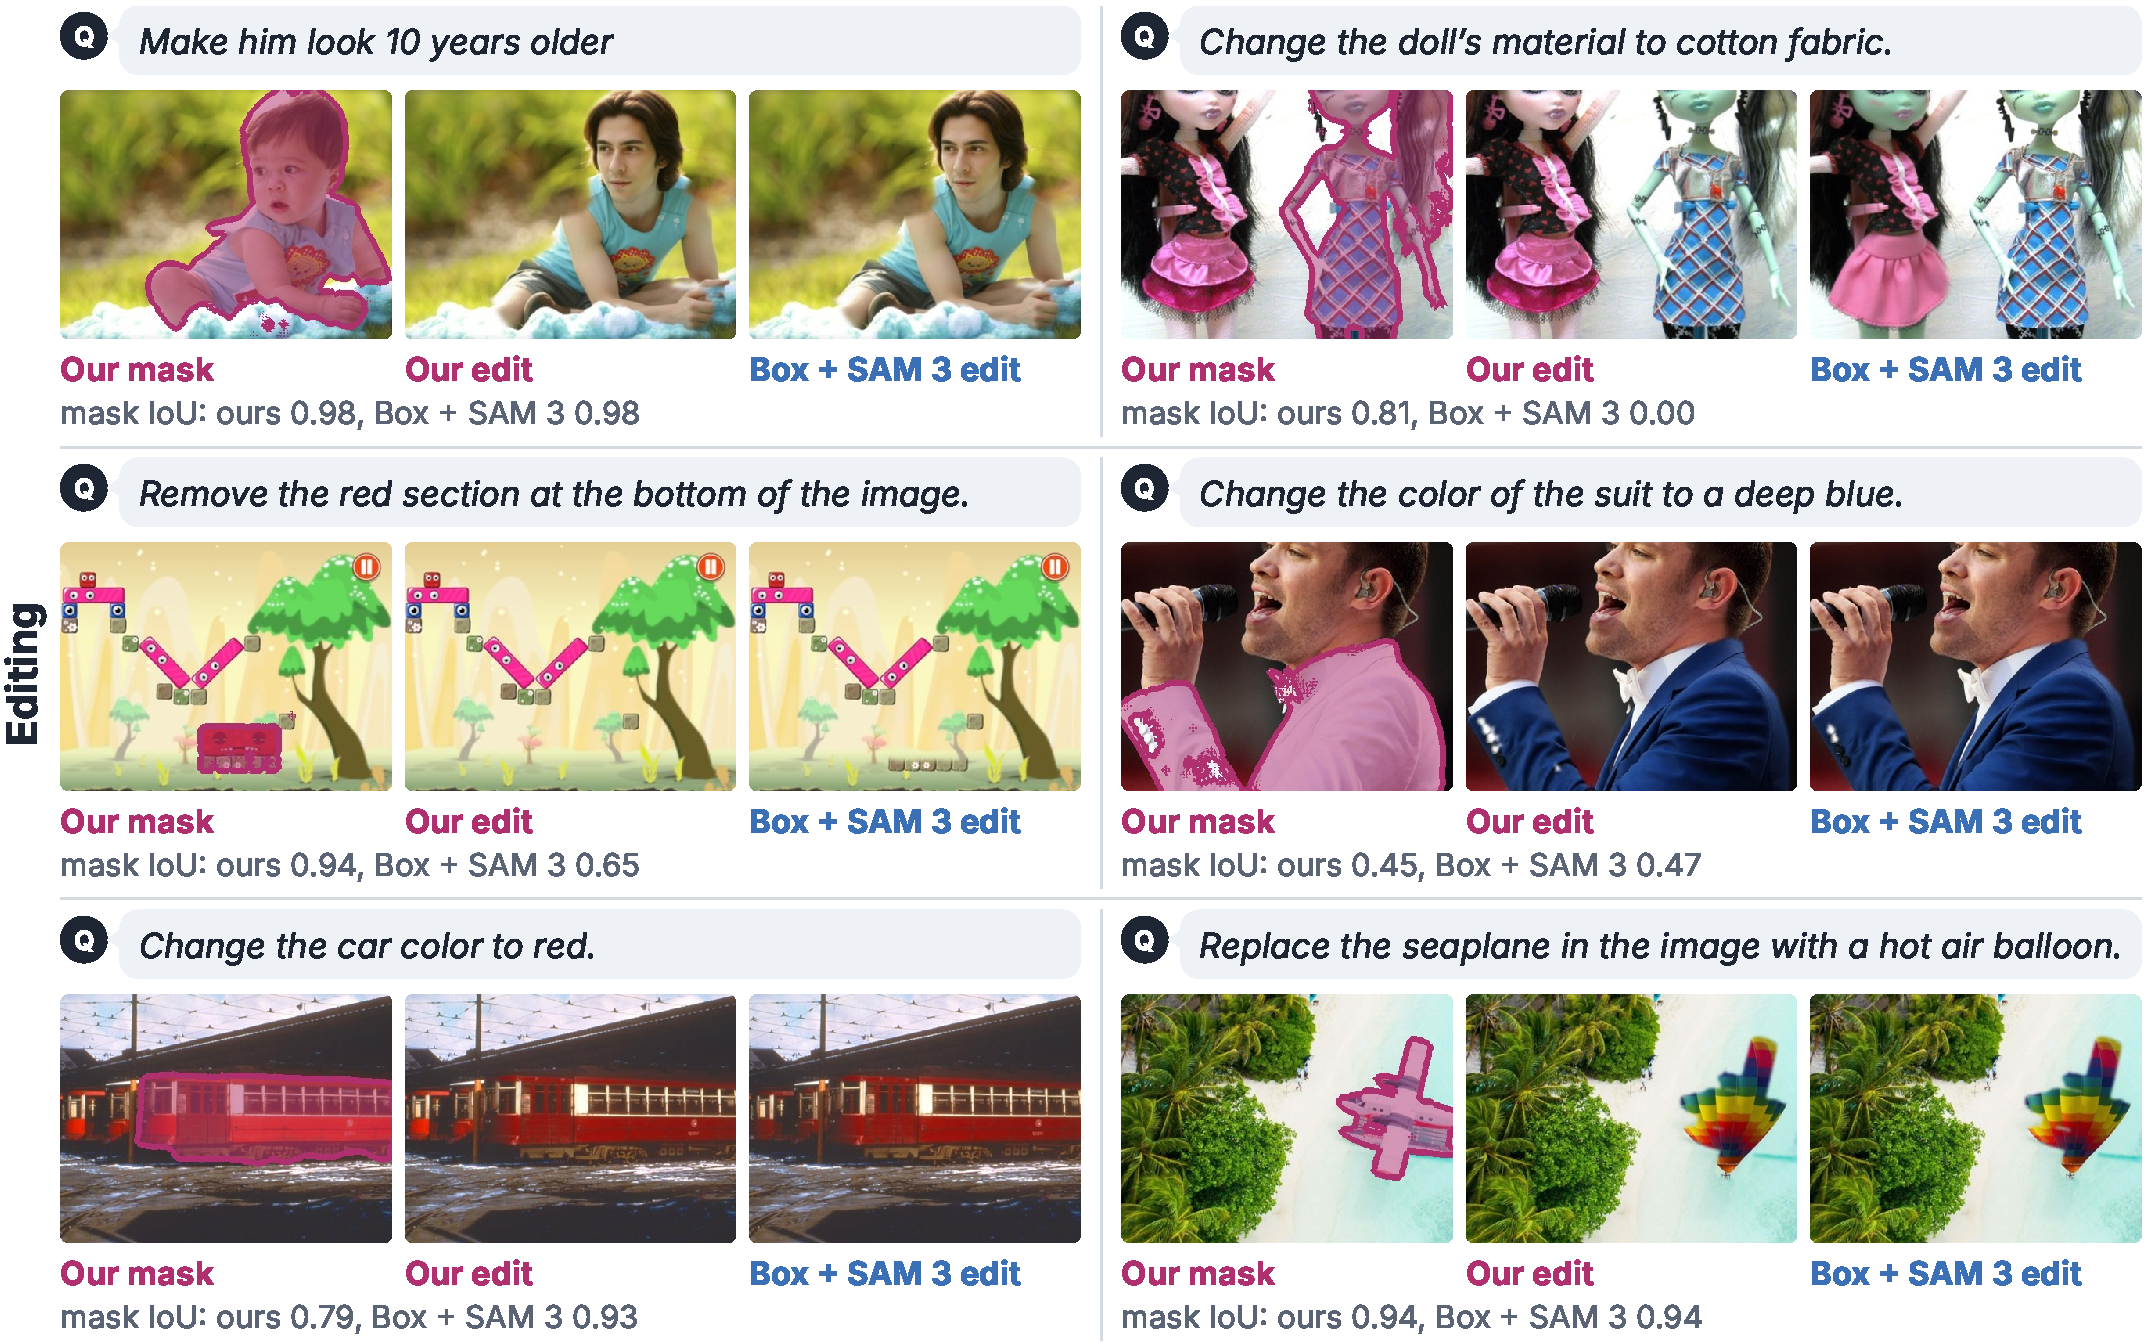
\includegraphics[width=\textwidth,height=0.9\textheight,keepaspectratio]{figures/qualitative/supp/edit_random.pdf}
\caption{\textbf{Editing: random examples.} A fixed-seed random sample of test queries, not selected for outcome. Our mask, the edit made with it, and the edit made with the Box + SAM\,3 mask (Qwen-Image-Edit).}
\label{fig:supp_edit_random}
\end{figure*}

\begin{figure*}[p]
\centering
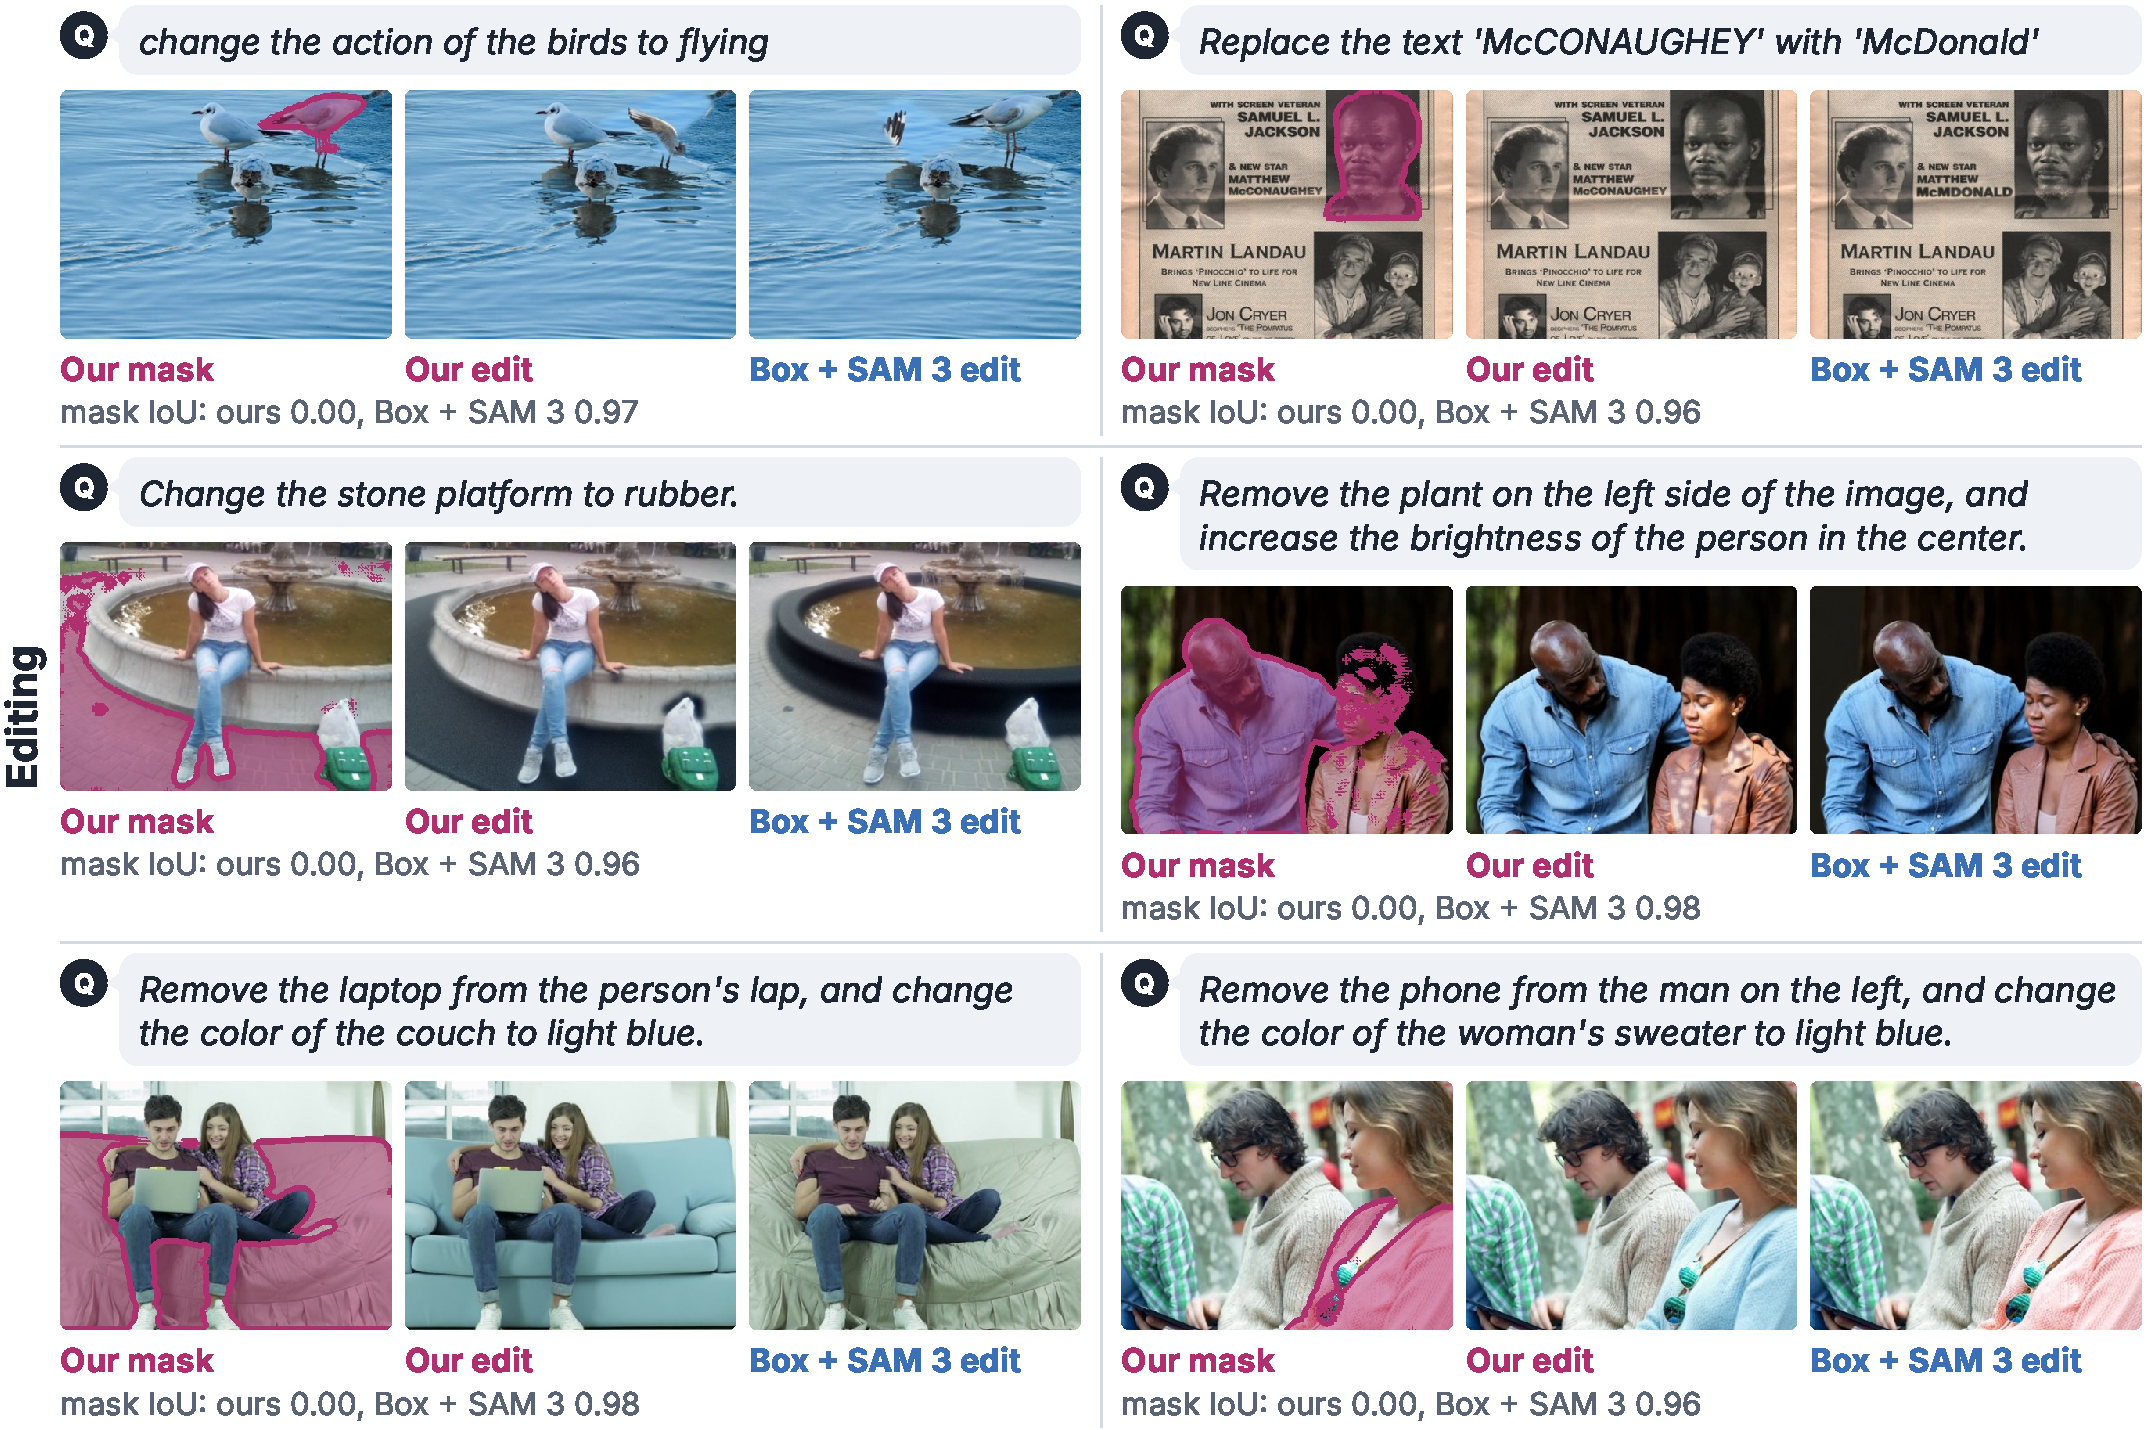
\includegraphics[width=\textwidth,height=0.9\textheight,keepaspectratio]{figures/qualitative/supp/edit_failures.pdf}
\caption{\textbf{Editing: failure cases.} The test queries where \ours{} falls furthest behind Box + SAM\,3. Our mask, the edit made with it, and the edit made with the Box + SAM\,3 mask (Qwen-Image-Edit).}
\label{fig:supp_edit_failures}
\end{figure*}


\end{document}
